\chapter{Methodology}

\section{Introduzione}
In questo capitolo viene esplorata la metodologia di lavoro adottata per lo sviluppo del progetto. Per la costruzione del prober universale è stato fatto uso del dataset ``Belief Bank'' \textcolor{red}{TODO:citazione}, che fornisce un insieme di affermazioni e la loro veridicità in diversi contesti. Sono stati presi in considerazione cinque diversi approcci metodologici per allineare lo spazio latente di un modello ``studente'' a quello di un modello ``insegnante''.
La prima fase del lavoro ha riguardato la preparazione del dataset e l'estrazione delle attivazioni interne dei modelli Qwen2.5-7B e Falcon3-7B-Base su tutti i layer e ogni tipologia di componente di un layer (attention, MLP, hidden states). Successivamente sono stati effettuati studi preliminari per valutare la capacità di ogni singolo componente di layer di discriminare tra affermazioni vere e allucinazioni, al fine di identificare i layer e le componenti più rilevanti per la costruzione del prober universale.
Sono state dunque calcolate alcune statistiche relative alle allucinazioni dei due modelli e tutte le attivazioni sono state preprocessate per essere utilizzate nei vari approcci metodologici.
In una prima fase è stato usato un approccio completamente lineare come baseline, per poi esplorare metodi più complessi che includono adattamenti non lineari tramite AdapterMLP, Encoder e AutoEncoder. Ogni metodologia è stata valutata in termini di prestazioni e capacità di trasferimento tra modelli diversi. 

\section{Dataset}

Il lavoro si basa su \textit{BeliefBank} \textcolor{red}{TODO: cita}, un dataset strutturato progettato per analizzare la consistenza e l'accuratezza delle credenze nei modelli linguistici pre-addestrati.

\subsection{BeliefBank}
\paragraph{Struttura del Dataset Originale}
Nella sua formulazione originale, BeliefBank si compone di due elementi distinti ma interconnessi:
\begin{itemize}
    \item \textbf{Vincoli (Constraints):} Un insieme di regole logiche formali, comprendenti implicazioni positive (es. $A \implies B$) e mutue esclusioni (es. $A \implies \neg B$). Questi vincoli sono stati estratti semi-automaticamente da knowledge base esterne quali ConceptNet e WordNet \textcolor{red}{TODO: cita}.
    \item \textbf{Fatti (Facts):} Un corpus di asserzioni vere o false generate istanziando i vincoli su un insieme di 85 entità (animali e piante). Le etichette di verità (``silver labels'') sono state ottenute annotando manualmente i nodi foglia del grafo e propagando la verità attraverso la rete dei vincoli.
\end{itemize}

\paragraph{Pre-elaborazione e Implementazione}
Per l'utilizzo nel progetto, i dati grezzi sono stati processati attraverso una pipeline dedicata che gestisce la trasformazione da rappresentazioni simboliche a linguaggio naturale e il bilanciamento delle classi.
I dati originali sono archiviati sotto forma di triple strutturate (soggetto, relazione, oggetto). La pipeline implementa un modulo di conversione che utilizza template predefiniti per trasformare queste triple in frasi di senso compiuto in lingua inglese. Per prevenire bias verso una specifica classe di risposta, il dataset viene esteso tramite una procedura di \textit{negation augmentation} generando sinteticamente la controparte negata di ogni fatto o implicazione presente, invertendo la label di verità associata. Questo approccio raddoppia efficacemente la dimensione del dataset e assicura che il modello sia esposto a una distribuzione bilanciata di etichette positive (yes) e negative (no). Ad ogni esempio è associato un identificativo univoco (\texttt{instance\_id}) per facilitare il tracciamento e l'analisi dei risultati.
Esempio di elementi del dataset dopo la pre-elaborazione:
\begin{itemize}
    \item \textbf{instance\_id}: 38
    \item \textbf{Question}: An albatross has a talon
    \item \textbf{Answer}: Yes
\end{itemize}

\subsection{Creazione dataset di attivazioni}
Una volta preparato il dataset di affermazioni e relative etichette di veridicità, il passo successivo è stato l'estrazione delle attivazioni interne dai modelli Qwen2.5-7B e Falcon3-7B-Base. 
Ogni esempio è preceduto da un prompt che viene fornito al modello di linguaggio per guidarne la risposta.
\textit{Answer the following question with just the essential information, without explanations}
Quindi il modello di linguaggio riceve in input il prompt seguito dalla domanda e deve rispondere con ``yes'' o ``no''.
Per ogni affermazione nel dataset, sono state registrate le attivazioni corrispondenti a tutti i layer e componenti (attention, MLP, hidden states) dei modelli. Queste attivazioni costituiscono la base dati su cui sono stati addestrati i vari prober per il rilevamento delle allucinazioni. Per verificare se il modello risponde correttamente o allucina è stata usata una semplice logica di matching tra la risposta generata e l'etichetta di veridicità associata all'affermazione nel dataset:
se la risposta reale (``yes'' o ``no'') è una substring (cioè è contenuta) nella risposta generata dal modello, allora l'affermazione è considerata vera (non allucinazione); altrimenti è considerata falsa (allucinazione).


\section{Studi preliminari}
\subsection{Statistiche sulle allucinazioni}
Prima di procedere con la costruzione del prober universale, sono state calcolate alcune statistiche relative alla frequenza delle allucinazioni nei modelli Qwen2.5-7B e Falcon3-7B-Base sul dataset Belief Bank.
Analizzando l'output dei modelli sul dataset Belief Bank, sono state calcolate le seguenti statistiche relative alle allucinazioni:
\begin{itemize}
    \item \textbf{Qwen2.5-7B}: su un totale di 27416 affermazioni, il modello ha generato 15728 allucinazioni
    \item \textbf{Falcon3-7B-Base}: su un totale di 27416 affermazioni, il modello ha generato 16499 allucinazioni
    \item \textbf{Allucinazioni comuni}: i due modelli condividono 12599 allucinazioni.
\end{itemize}
I risultati suggeriscono che i modelli si comportano in modo molto simile, il che indica che le allucinazioni potrebbero essere legate a caratteristiche intrinseche nei modelli di linguaggio (e dunque la costruzione di un prober universale potrebbe essere possibile).

\subsection{Studio delle singole componenti di layer}

Per valutare la capacità discriminativa delle diverse componenti di layer (attention, MLP, hidden states) dei modelli Qwen2.5-7B e Falcon3-7B-Base nel rilevamento delle allucinazioni, sono stati condotti esperimenti sistematici su ciascun layer e tipologia di attivazione. In particolare, per ogni layer e componente, sono state estratte le attivazioni corrispondenti e utilizzate come input per addestrare un classificatore Logistic Regression, con l’obiettivo di distinguere tra affermazioni vere e allucinazioni.

La pipeline sperimentale prevede:
\begin{itemize}
\item Estrazione delle attivazioni per ogni layer e componente (attention, MLP, hidden) dai modelli su tutto il dataset.
\item Suddivisione del dataset in training e test set, mantenendo la stessa suddivisione per tutti gli esperimenti.
\item Normalizzazione delle attivazioni tramite StandardScaler.
\item Addestramento di un classificatore Logistic Regression per ciascuna combinazione layer/componente.
\item Valutazione delle prestazioni tramite metriche di accuratezza e F1-score.
\item Ordinamento dei layer in base alle performance ottenute, per identificare quelli più rilevanti.
\end{itemize}

I risultati mostrano che alcune componenti e layer sono particolarmente efficaci nel discriminare le allucinazioni, evidenziando la presenza di pattern informativi specifici nelle attivazioni interne dei modelli. Tutti i risultati sono stati salvati e ordinati in formato JSON per facilitare l’analisi comparativa tra modelli e componenti.

\begin{table}[H]
\centering
\caption{Risultati completi per Qwen2.5-7B (ordinati per performance decrescente)}
\label{tab:qwen-results}
\resizebox{\textwidth}{!}{%
\begin{tabular}{c|ccc|ccc|ccc}
\toprule
 & \multicolumn{3}{c|}{\textbf{Attention (Attn)}} & \multicolumn{3}{c|}{\textbf{MLP}} & \multicolumn{3}{c}{\textbf{Hidden}} \\
\textbf{Rank} & \textbf{Lyr} & \textbf{Acc} & \textbf{F1} & \textbf{Lyr} & \textbf{Acc} & \textbf{F1} & \textbf{Lyr} & \textbf{Acc} & \textbf{F1} \\
\midrule
1 & 16 & 0.9866 & 0.9885 & 20 & 0.9886 & 0.9902 & 18 & 0.9904 & 0.9918 \\
2 & 18 & 0.9861 & 0.9881 & 16 & 0.9884 & 0.9901 & 20 & 0.9894 & 0.9909 \\
3 & 19 & 0.9859 & 0.9879 & 18 & 0.9883 & 0.9900 & 19 & 0.9892 & 0.9907 \\
4 & 15 & 0.9858 & 0.9878 & 19 & 0.9878 & 0.9896 & 16 & 0.9883 & 0.9900 \\
5 & 21 & 0.9850 & 0.9872 & 21 & 0.9875 & 0.9893 & 21 & 0.9882 & 0.9899 \\
6 & 11 & 0.9847 & 0.9868 & 12 & 0.9872 & 0.9891 & 17 & 0.9877 & 0.9895 \\
7 & 12 & 0.9846 & 0.9867 & 17 & 0.9871 & 0.9889 & 22 & 0.9875 & 0.9893 \\
8 & 10 & 0.9841 & 0.9863 & 14 & 0.9861 & 0.9881 & 23 & 0.9874 & 0.9891 \\
9 & 8 & 0.9838 & 0.9861 & 15 & 0.9861 & 0.9881 & 14 & 0.9871 & 0.9889 \\
10 & 17 & 0.9838 & 0.9861 & 10 & 0.9860 & 0.9880 & 15 & 0.9871 & 0.9889 \\
11 & 13 & 0.9832 & 0.9856 & 9 & 0.9855 & 0.9876 & 24 & 0.9869 & 0.9887 \\
12 & 14 & 0.9831 & 0.9855 & 11 & 0.9853 & 0.9874 & 13 & 0.9864 & 0.9883 \\
13 & 20 & 0.9831 & 0.9855 & 13 & 0.9853 & 0.9874 & 11 & 0.9863 & 0.9882 \\
14 & 25 & 0.9830 & 0.9854 & 8 & 0.9850 & 0.9872 & 12 & 0.9863 & 0.9882 \\
15 & 6 & 0.9825 & 0.9849 & 22 & 0.9850 & 0.9872 & 25 & 0.9860 & 0.9880 \\
16 & 3 & 0.9822 & 0.9848 & 23 & 0.9848 & 0.9869 & 7 & 0.9859 & 0.9879 \\
17 & 24 & 0.9820 & 0.9845 & 6 & 0.9843 & 0.9865 & 26 & 0.9859 & 0.9879 \\
18 & 22 & 0.9815 & 0.9841 & 7 & 0.9835 & 0.9858 & 10 & 0.9852 & 0.9873 \\
19 & 23 & 0.9808 & 0.9835 & 24 & 0.9835 & 0.9858 & 9 & 0.9847 & 0.9869 \\
20 & 7 & 0.9801 & 0.9829 & 27 & 0.9832 & 0.9856 & 27 & 0.9847 & 0.9868 \\
21 & 26 & 0.9799 & 0.9828 & 25 & 0.9831 & 0.9855 & 6 & 0.9840 & 0.9862 \\
22 & 4 & 0.9795 & 0.9823 & 26 & 0.9819 & 0.9845 & 8 & 0.9840 & 0.9862 \\
23 & 9 & 0.9793 & 0.9823 & 4 & 0.9808 & 0.9835 & 5 & 0.9829 & 0.9853 \\
24 & 5 & 0.9782 & 0.9813 & 5 & 0.9791 & 0.9820 & 4 & 0.9824 & 0.9849 \\
25 & 2 & 0.9774 & 0.9806 & 3 & 0.9776 & 0.9807 & 3 & 0.9809 & 0.9836 \\
26 & 27 & 0.9770 & 0.9803 & 0 & 0.9734 & 0.9771 & 2 & 0.9780 & 0.9811 \\
27 & 1 & 0.9731 & 0.9769 & 2 & 0.9712 & 0.9752 & 0 & 0.9743 & 0.9779 \\
28 & 0 & 0.9725 & 0.9764 & 1 & 0.9653 & 0.9701 & 1 & 0.9736 & 0.9773 \\
\bottomrule
\end{tabular}%
}
\end{table}



\begin{table}[H]
\centering
\caption{Risultati completi per Falcon3-7B-Base (ordinati per performance decrescente)}
\label{tab:falcon-results}
\resizebox{\textwidth}{!}{%
\begin{tabular}{c|ccc|ccc|ccc}
\toprule
 & \multicolumn{3}{c|}{\textbf{Attention (Attn)}} & \multicolumn{3}{c|}{\textbf{MLP}} & \multicolumn{3}{c}{\textbf{Hidden}} \\
\textbf{Rank} & \textbf{Lyr} & \textbf{Acc} & \textbf{F1} & \textbf{Lyr} & \textbf{Acc} & \textbf{F1} & \textbf{Lyr} & \textbf{Acc} & \textbf{F1} \\
\midrule
1 & 2 & 0.8118 & 0.8334 & 10 & 0.7897 & 0.8155 & 3 & 0.7938 & 0.8189 \\
2 & 12 & 0.8108 & 0.8324 & 12 & 0.7880 & 0.8125 & 19 & 0.7903 & 0.8153 \\
3 & 7 & 0.8091 & 0.8310 & 11 & 0.7876 & 0.8134 & 2 & 0.7900 & 0.8157 \\
4 & 17 & 0.8084 & 0.8310 & 6 & 0.7867 & 0.8120 & 5 & 0.7887 & 0.8135 \\
5 & 27 & 0.8083 & 0.8306 & 7 & 0.7849 & 0.8121 & 8 & 0.7886 & 0.8141 \\
6 & 13 & 0.8069 & 0.8294 & 5 & 0.7842 & 0.8104 & 13 & 0.7886 & 0.8134 \\
7 & 20 & 0.8063 & 0.8287 & 21 & 0.7840 & 0.8088 & 20 & 0.7883 & 0.8132 \\
8 & 10 & 0.8061 & 0.8283 & 4 & 0.7836 & 0.8095 & 14 & 0.7878 & 0.8123 \\
9 & 1 & 0.8049 & 0.8267 & 20 & 0.7835 & 0.8090 & 18 & 0.7871 & 0.8103 \\
10 & 25 & 0.8044 & 0.8283 & 15 & 0.7832 & 0.8090 & 4 & 0.7869 & 0.8118 \\
11 & 22 & 0.8041 & 0.8276 & 25 & 0.7829 & 0.8094 & 26 & 0.7866 & 0.8131 \\
12 & 24 & 0.8029 & 0.8257 & 13 & 0.7827 & 0.8084 & 9 & 0.7863 & 0.8112 \\
13 & 8 & 0.8023 & 0.8250 & 16 & 0.7825 & 0.8080 & 15 & 0.7859 & 0.8117 \\
14 & 19 & 0.8018 & 0.8246 & 18 & 0.7815 & 0.8067 & 12 & 0.7858 & 0.8107 \\
15 & 3 & 0.8016 & 0.8244 & 14 & 0.7809 & 0.8063 & 25 & 0.7852 & 0.8108 \\
16 & 4 & 0.8009 & 0.8240 & 9 & 0.7807 & 0.8070 & 17 & 0.7850 & 0.8105 \\
17 & 9 & 0.8005 & 0.8233 & 27 & 0.7805 & 0.8056 & 10 & 0.7846 & 0.8101 \\
18 & 11 & 0.8000 & 0.8223 & 19 & 0.7803 & 0.8069 & 21 & 0.7844 & 0.8094 \\
19 & 0 & 0.7989 & 0.8188 & 2 & 0.7799 & 0.8053 & 23 & 0.7844 & 0.8091 \\
20 & 16 & 0.7988 & 0.8216 & 3 & 0.7796 & 0.8051 & 24 & 0.7844 & 0.8103 \\
21 & 14 & 0.7987 & 0.8210 & 24 & 0.7795 & 0.8054 & 22 & 0.7843 & 0.8099 \\
22 & 21 & 0.7981 & 0.8210 & 8 & 0.7791 & 0.8051 & 6 & 0.7840 & 0.8097 \\
23 & 23 & 0.7981 & 0.8221 & 23 & 0.7786 & 0.8036 & 1 & 0.7830 & 0.8082 \\
24 & 6 & 0.7979 & 0.8214 & 17 & 0.7778 & 0.8042 & 11 & 0.7830 & 0.8085 \\
25 & 15 & 0.7970 & 0.8194 & 1 & 0.7711 & 0.7966 & 27 & 0.7819 & 0.8085 \\
26 & 5 & 0.7959 & 0.8186 & 22 & 0.7697 & 0.7960 & 7 & 0.7818 & 0.8081 \\
27 & 18 & 0.7947 & 0.8181 & 26 & 0.7675 & 0.7948 & 16 & 0.7810 & 0.8056 \\
28 & 26 & 0.7929 & 0.8164 & 0 & 0.7584 & 0.7860 & 0 & 0.7627 & 0.7898 \\
\bottomrule
\end{tabular}%
}
\end{table}

Successivamente è stata effettuata un'analisi relativa alla distribuzione di allucinazioni e risposte corrette nello spazio delle attivazioni. Affinchè fosse possibile visualizzare le attivazioni in uno spazio bidimensionale, è stata applicata la tecnica di riduzione della dimensionalità PCA (Principal Component Analysis).

\begin{figure}[H]
    \centering
    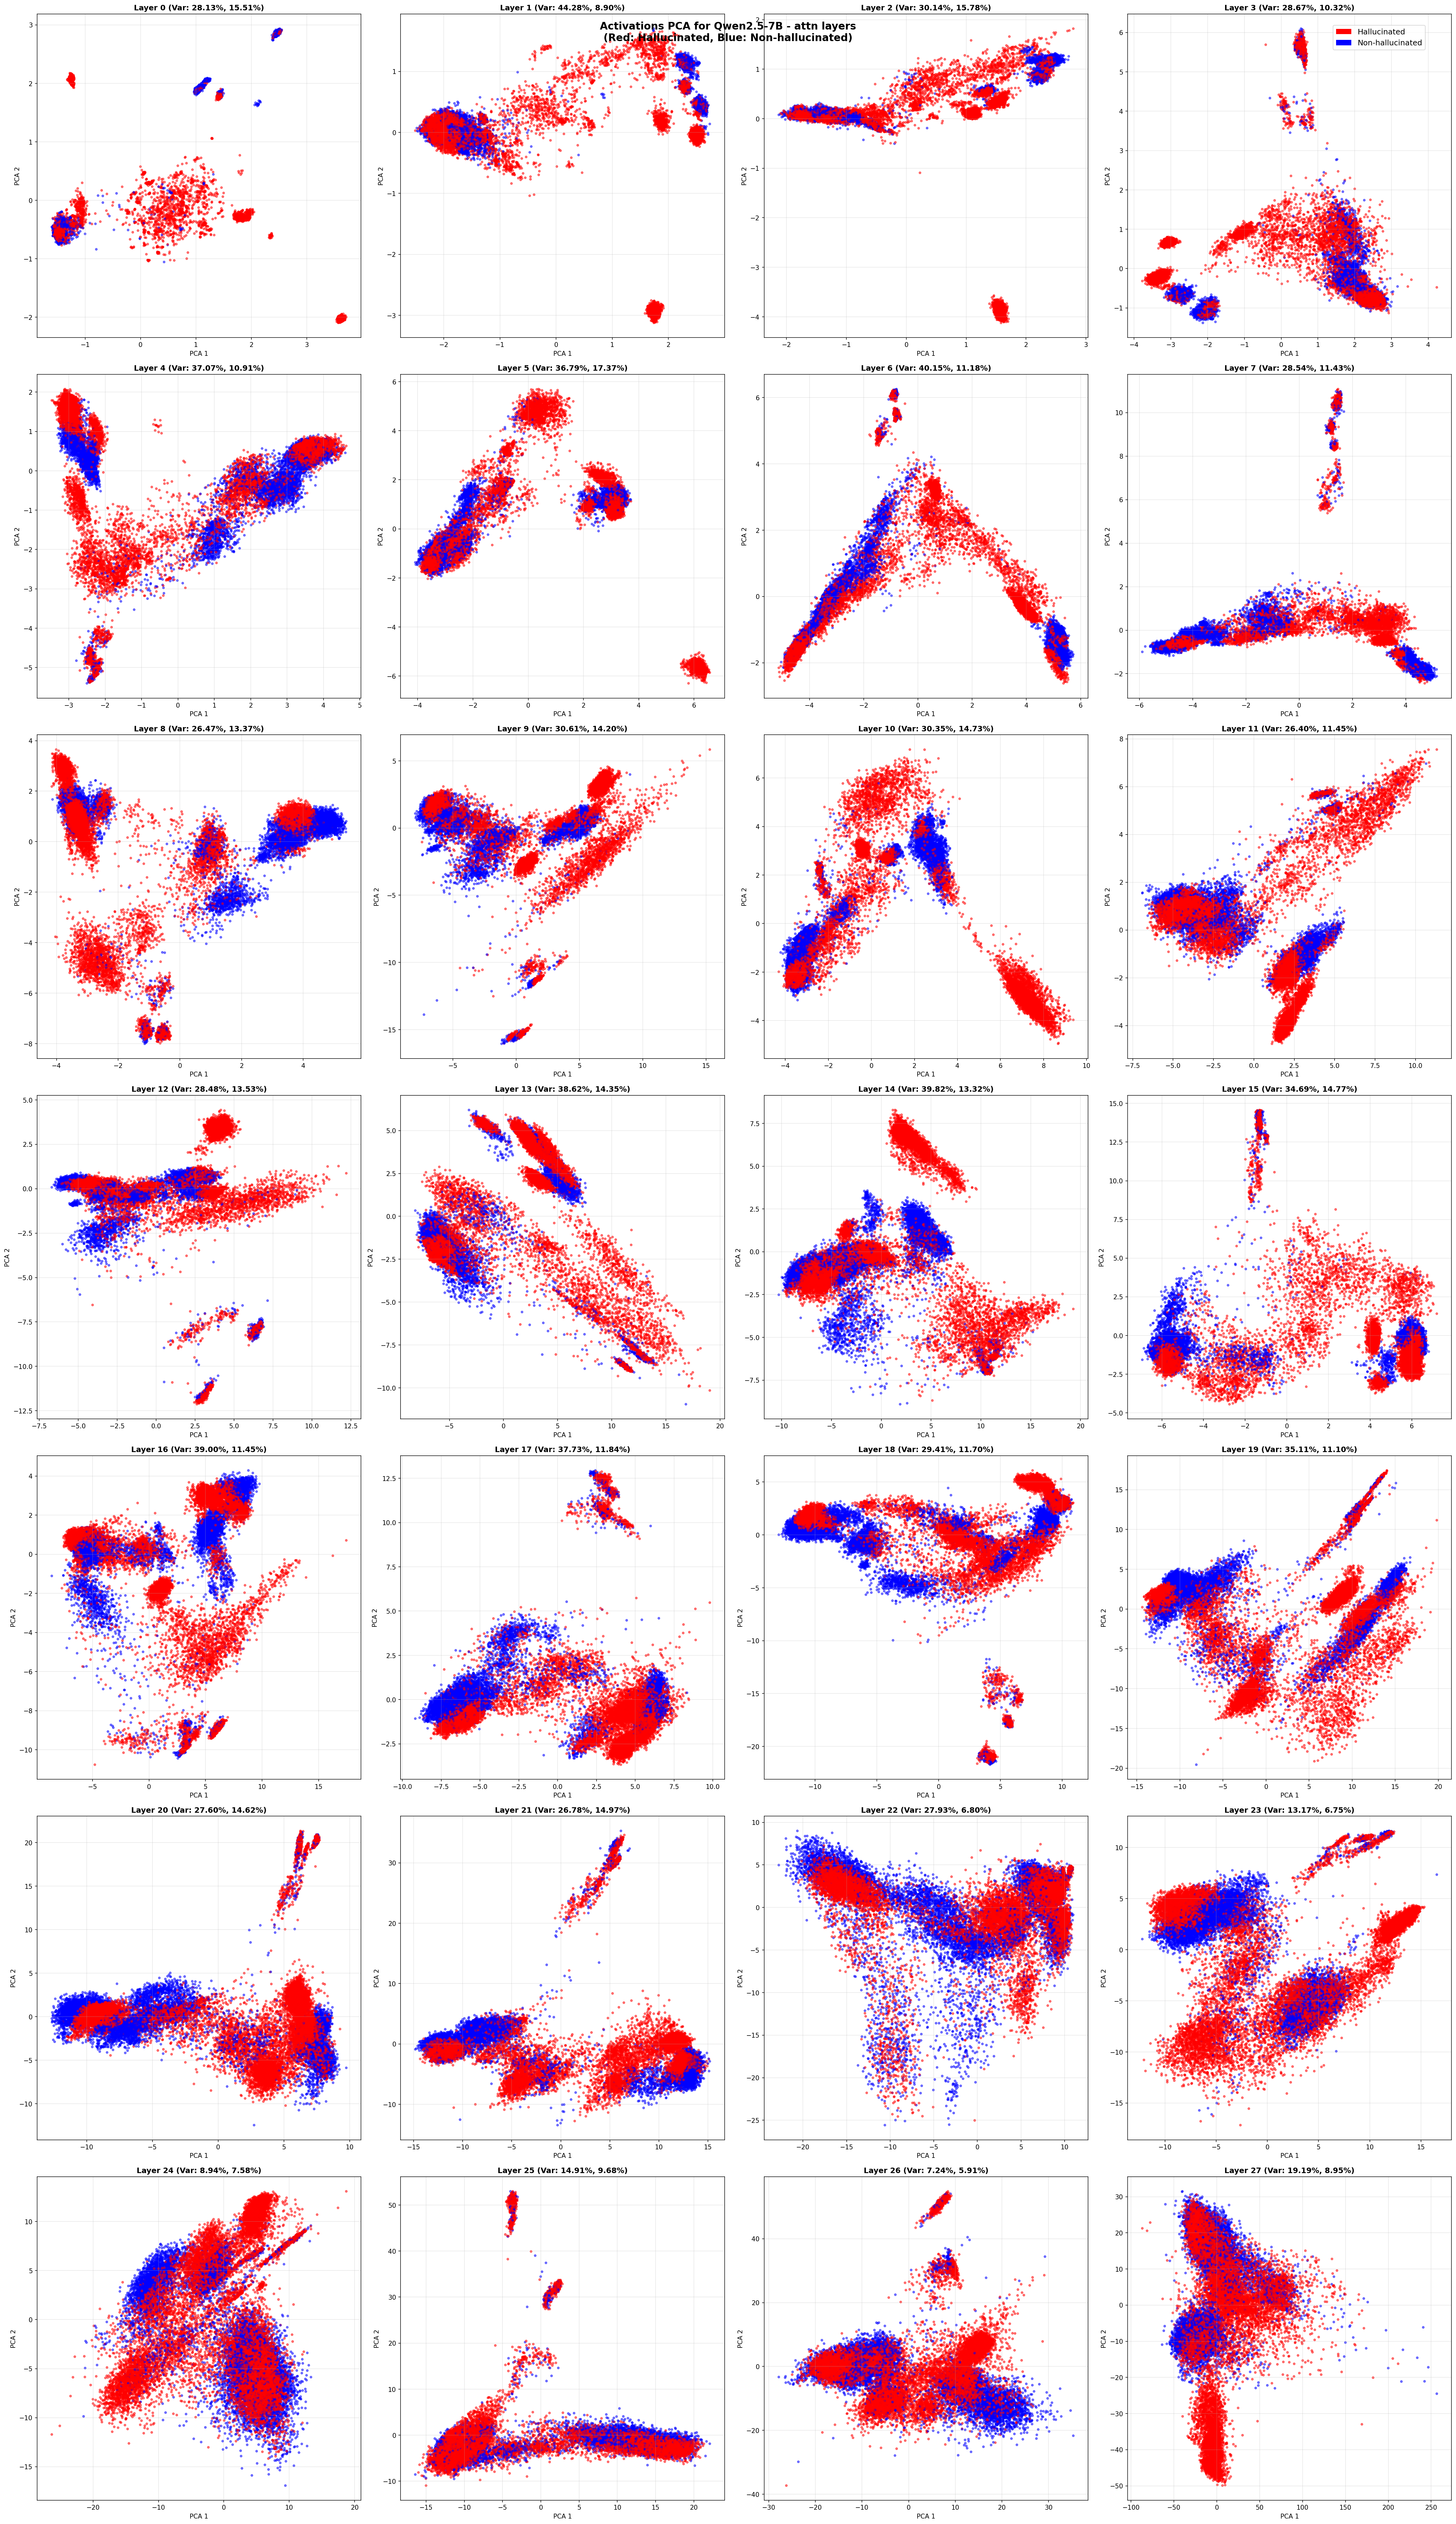
\includegraphics[width=\textwidth, height=0.8\textheight, keepaspectratio]{images/PCA_Plots/Qwen2.5-7B_belief_bank_attn_activations_PCA.png}
    \caption{PCA delle attivazioni Attention del layer di Qwen2.5-7B}
    \label{fig:qwen-pca-attn}
\end{figure}

\begin{figure}[H]
    \centering
    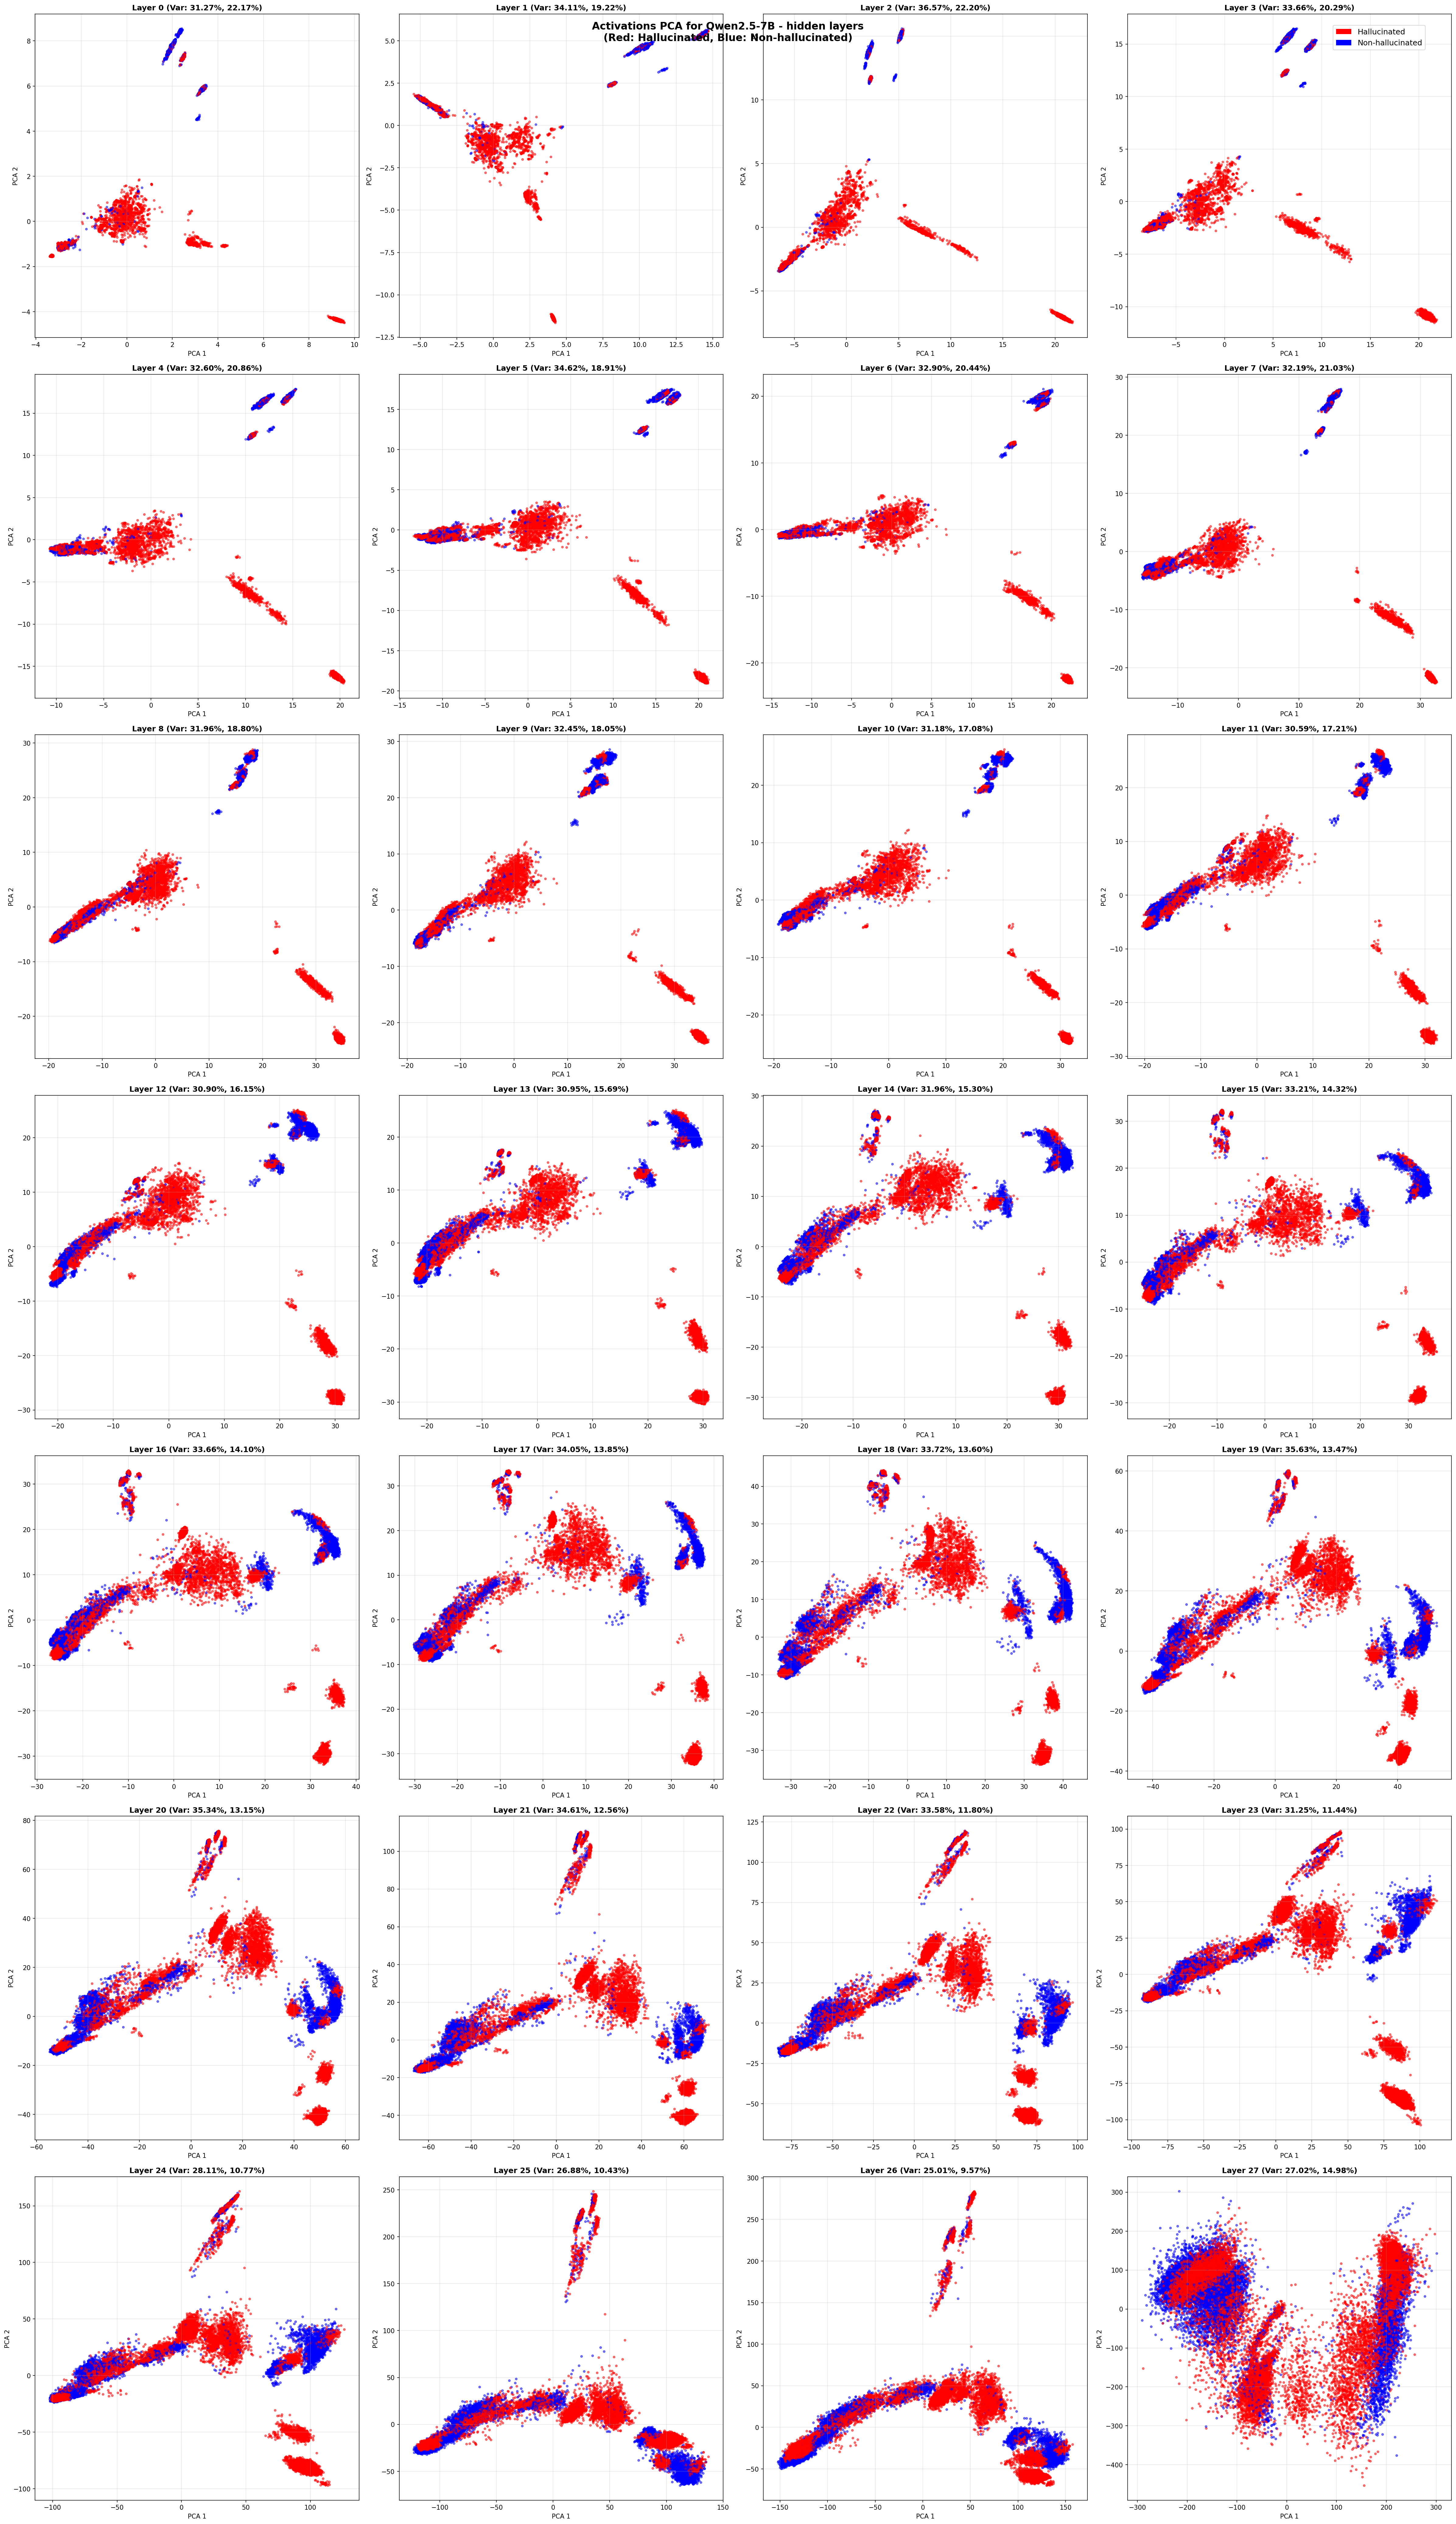
\includegraphics[width=\textwidth, height=0.8\textheight, keepaspectratio]{images/PCA_Plots/Qwen2.5-7B_belief_bank_hidden_activations_PCA.png}
    \caption{PCA delle attivazioni Hidden del layer di Qwen2.5-7B}
    \label{fig:qwen-pca-hidden}
\end{figure}

\begin{figure}[H]
    \centering
    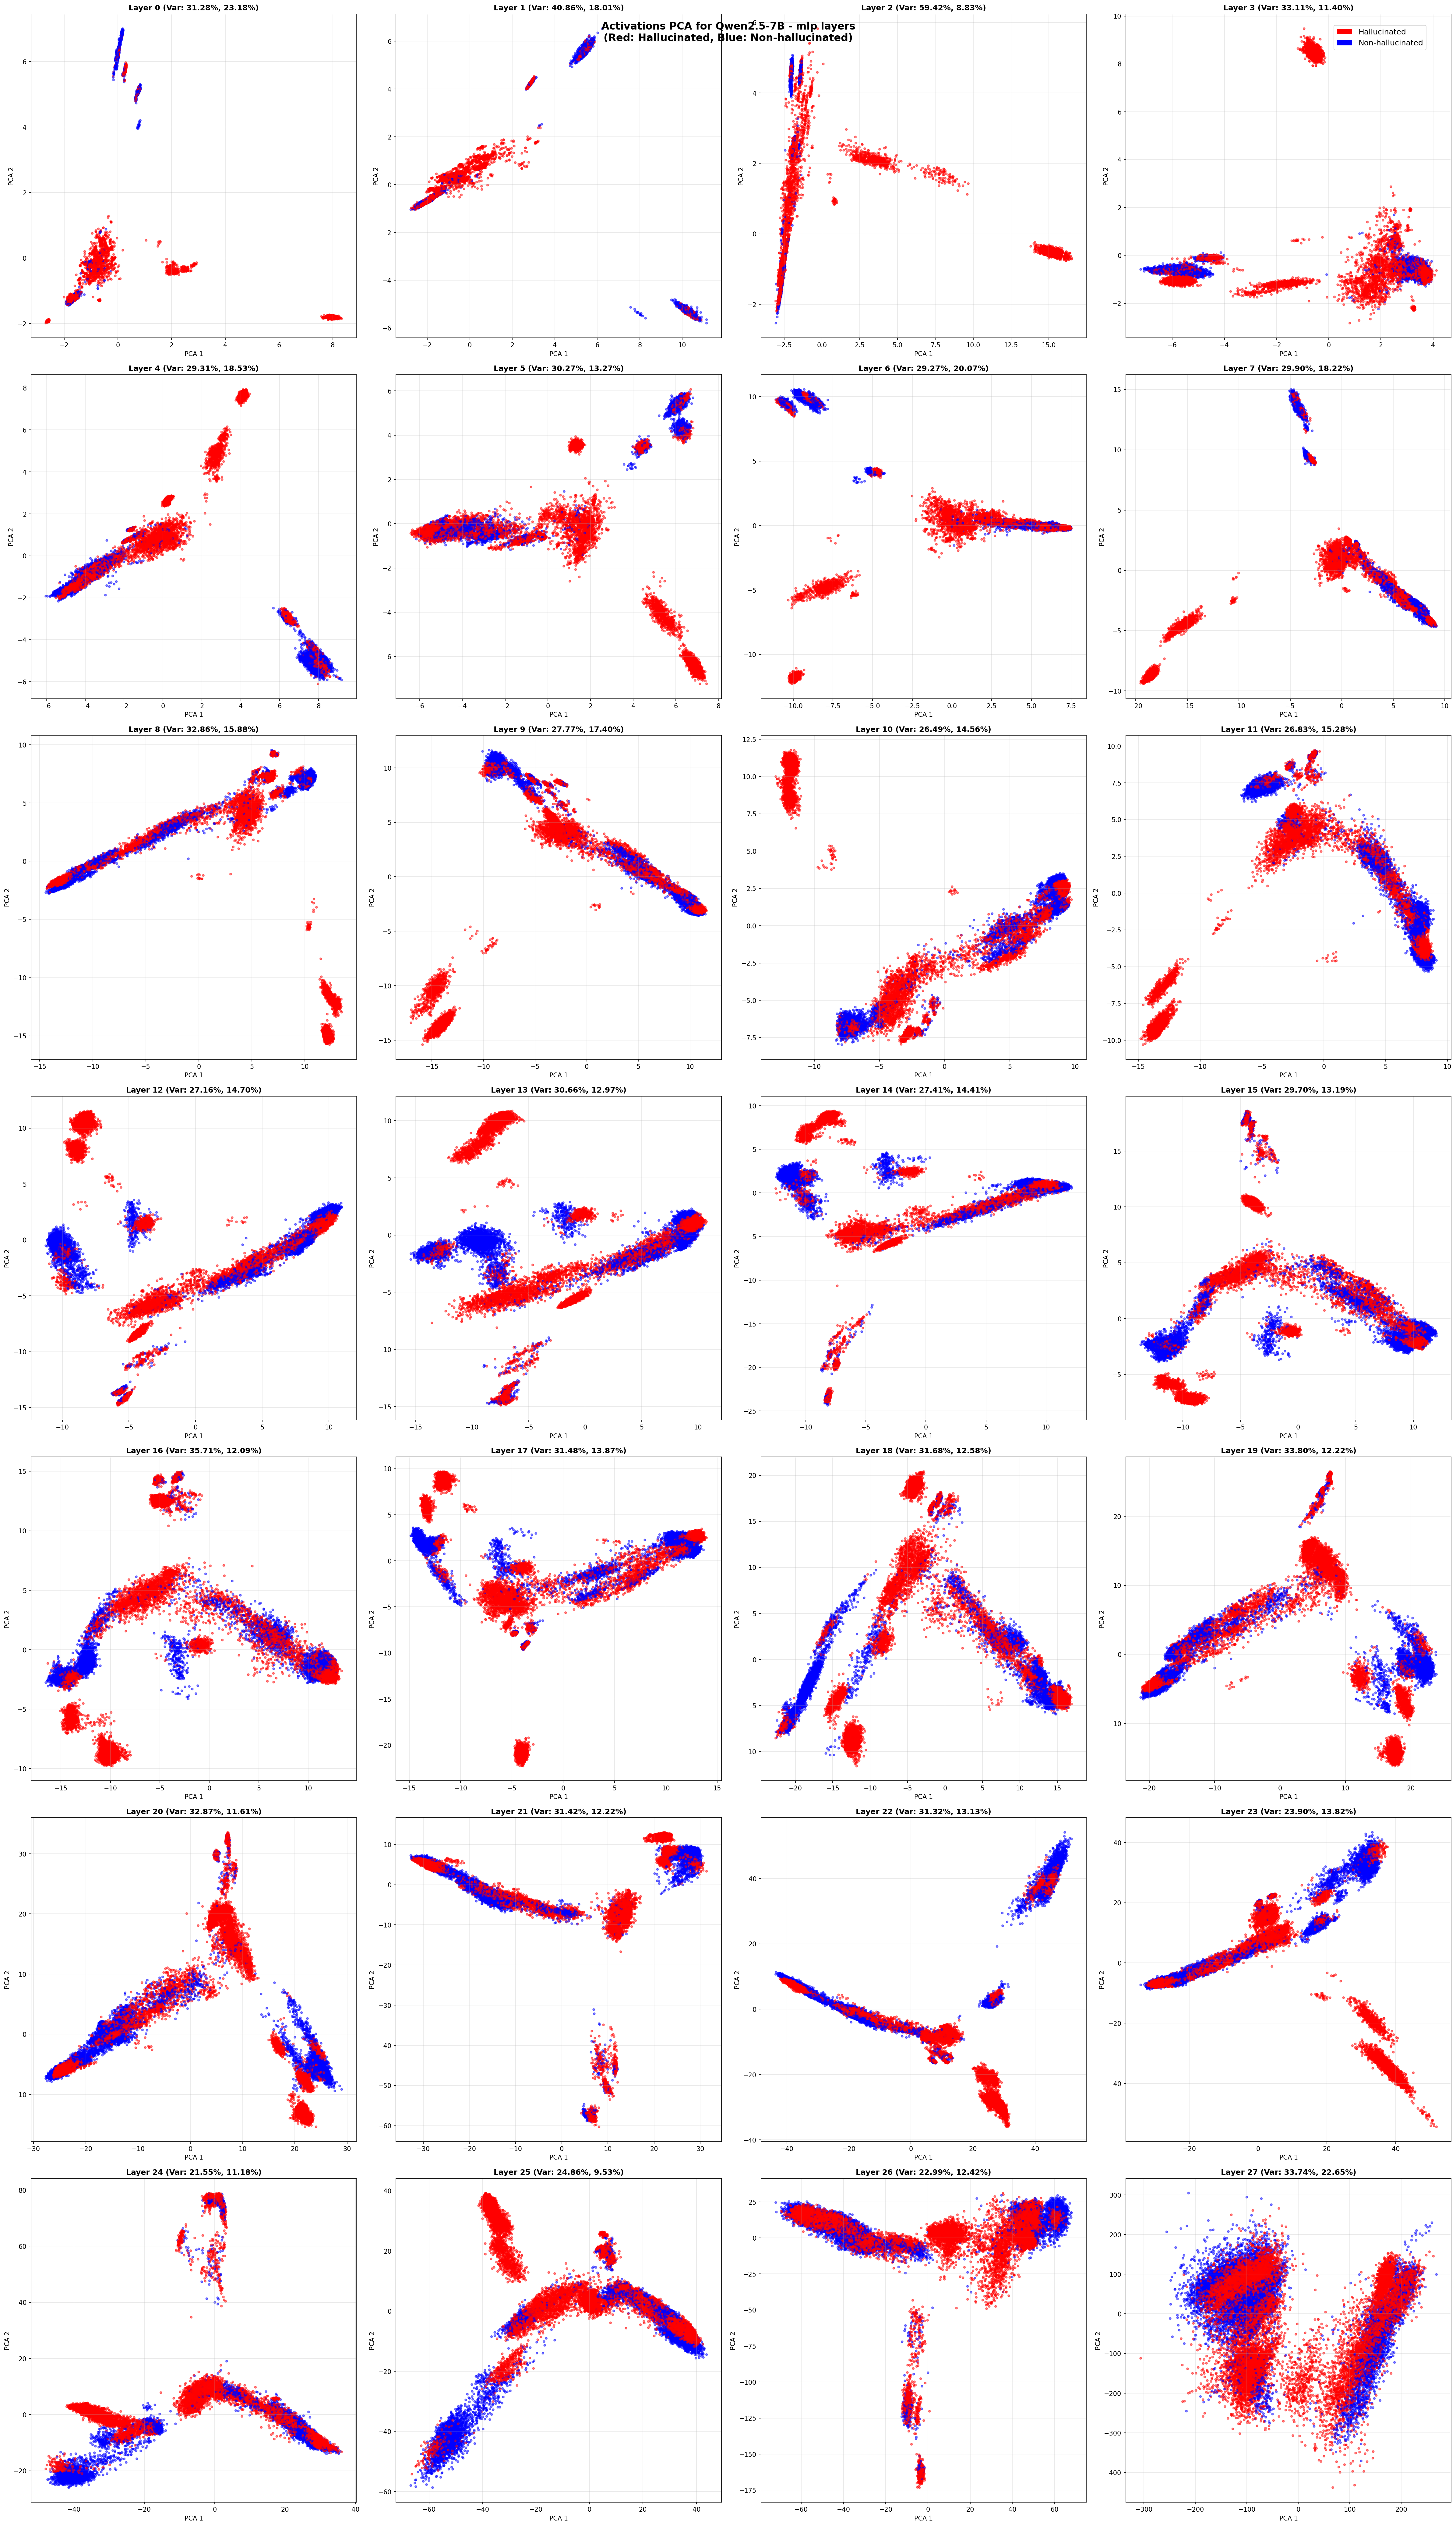
\includegraphics[width=\textwidth, height=0.8\textheight, keepaspectratio]{images/PCA_Plots/Qwen2.5-7B_belief_bank_mlp_activations_PCA.png}
    \caption{PCA delle attivazioni MLP del layer di Qwen2.5-7B}
    \label{fig:qwen-pca-mlp}
\end{figure}


\begin{figure}[H]
    \centering
    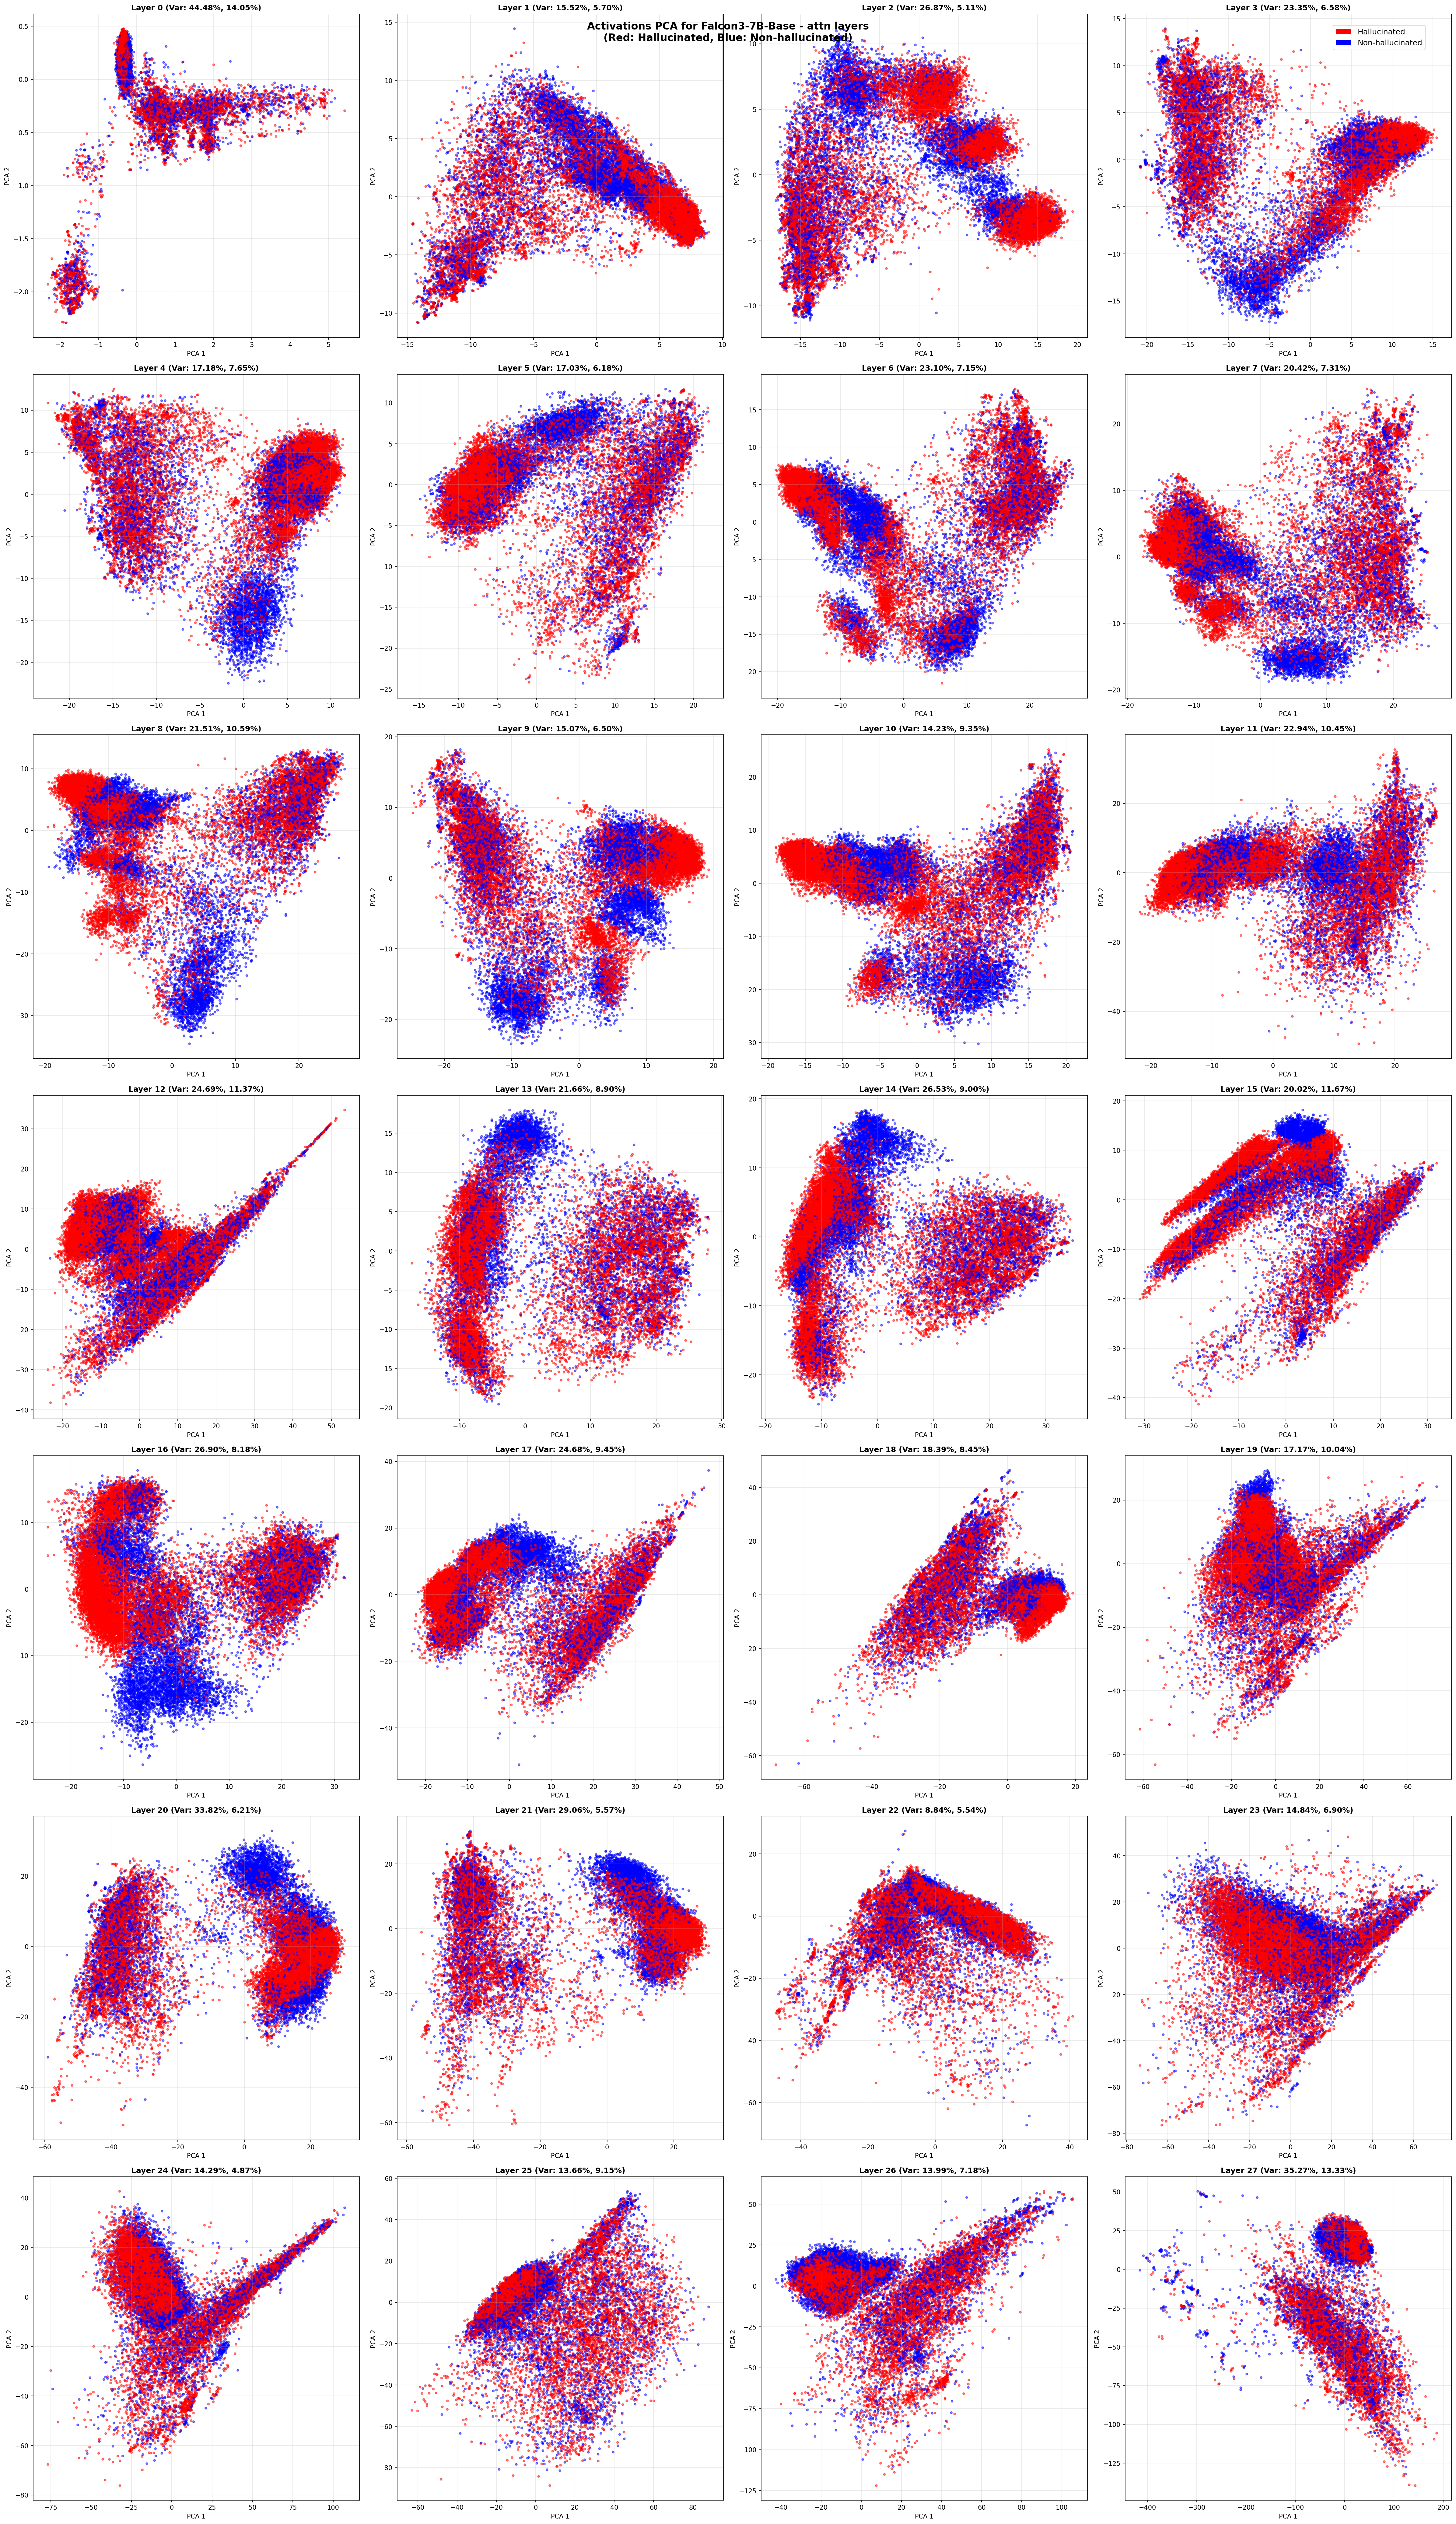
\includegraphics[width=\textwidth, height=0.8\textheight, keepaspectratio]{images/PCA_Plots/Falcon3-7B-Base_belief_bank_attn_activations_PCA.png}
    \caption{PCA delle attivazioni Attention del layer di Falcon3-7B-Base}
    \label{fig:falcon-pca-attn}
\end{figure}

\begin{figure}[H]
    \centering
    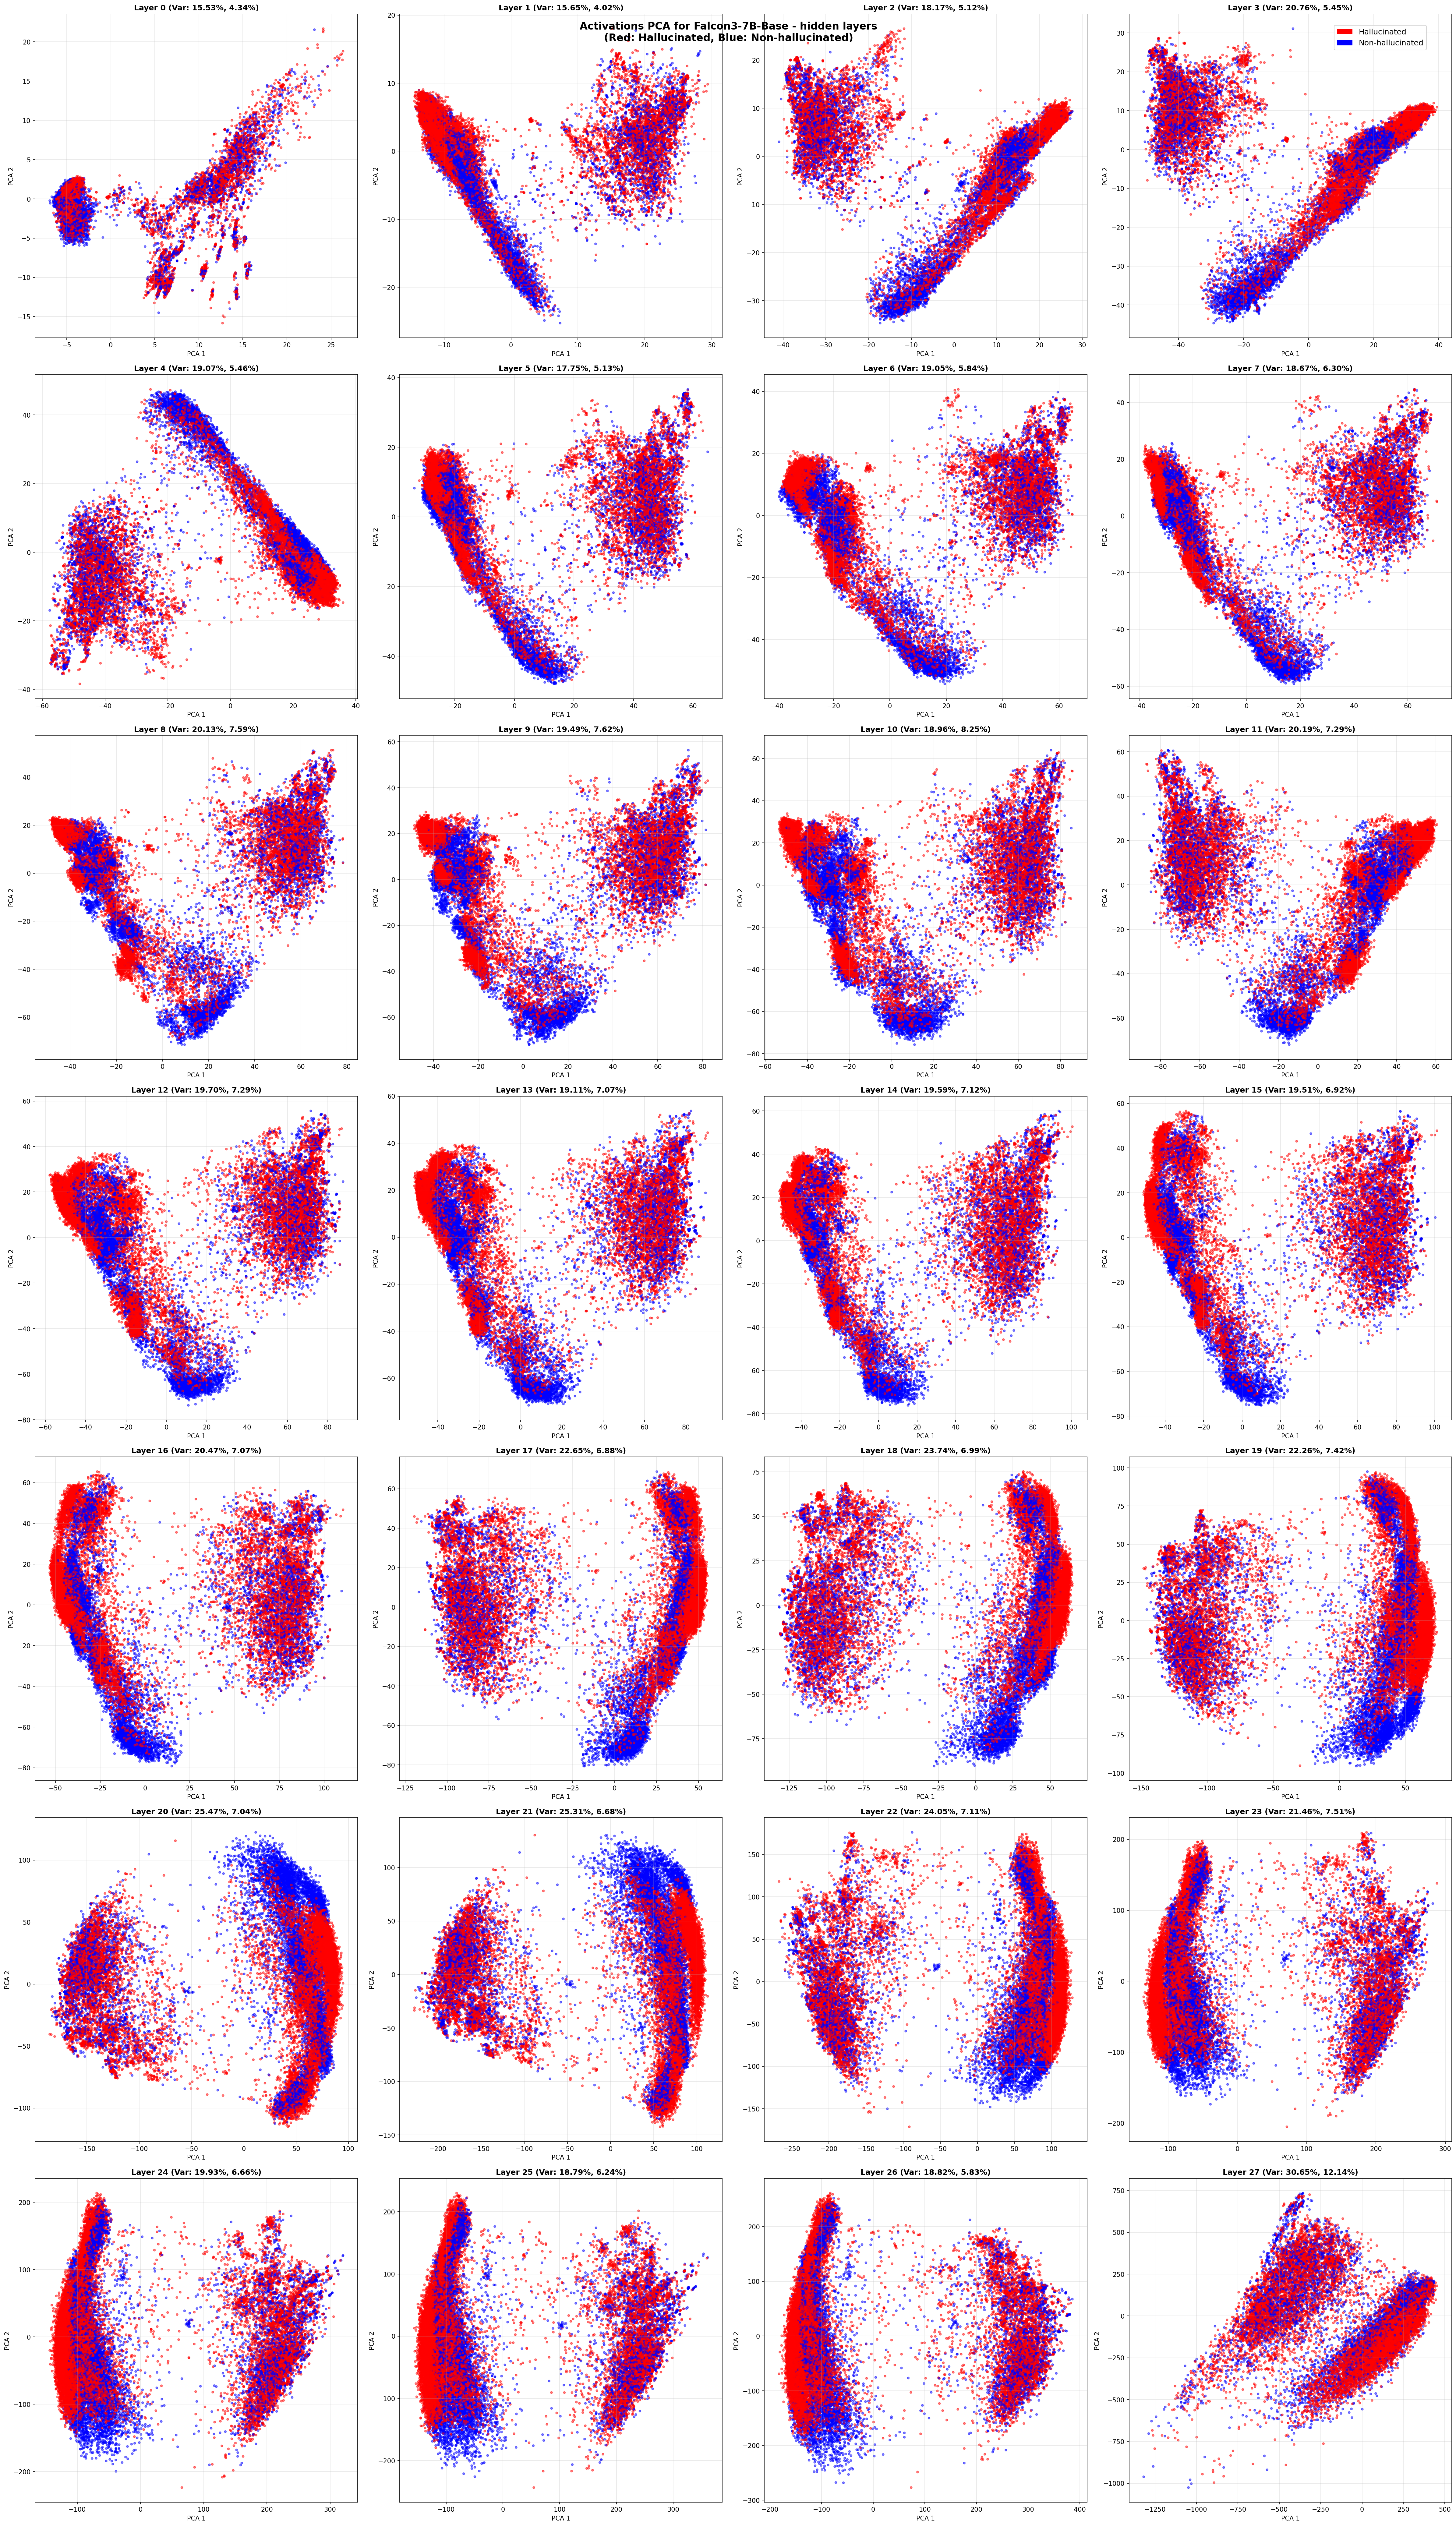
\includegraphics[width=\textwidth, height=0.8\textheight, keepaspectratio]{images/PCA_Plots/Falcon3-7B-Base_belief_bank_hidden_activations_PCA.png}
    \caption{PCA delle attivazioni Hidden del layer di Falcon3-7B-Base}
    \label{fig:falcon-pca-hidden}
\end{figure}

\begin{figure}[H]
    \centering
    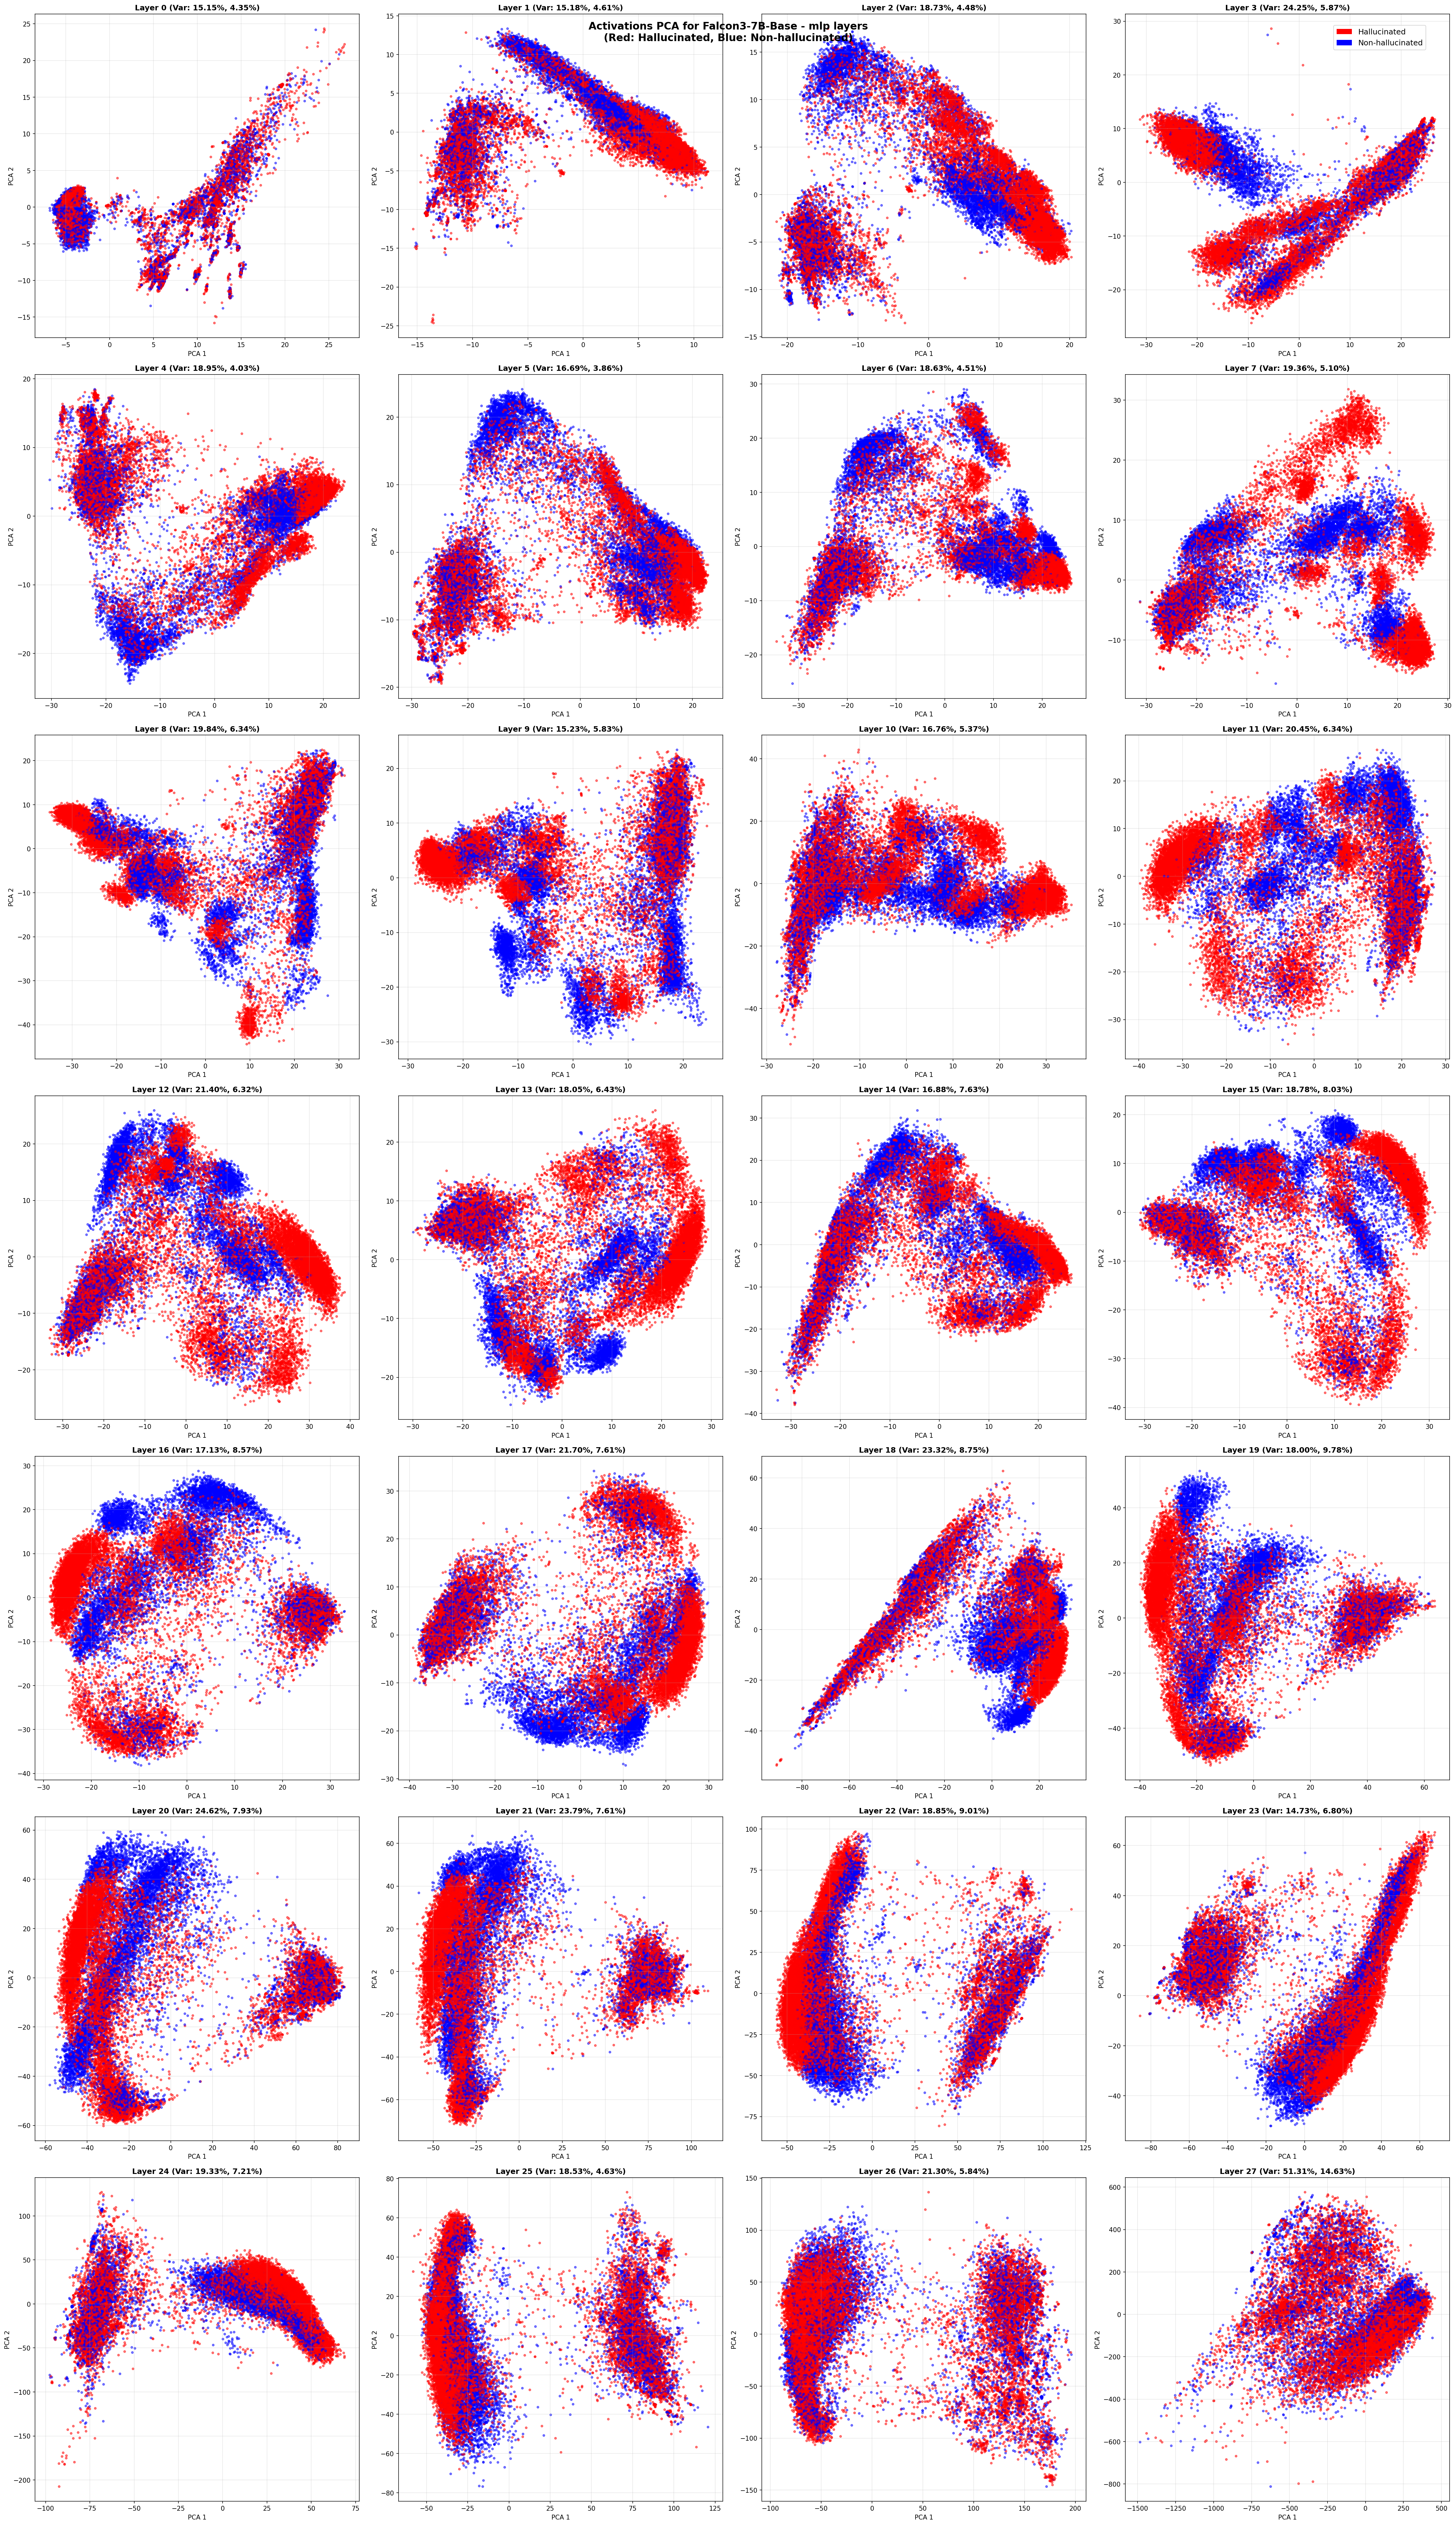
\includegraphics[width=\textwidth, height=0.8\textheight, keepaspectratio]{images/PCA_Plots/Falcon3-7B-Base_belief_bank_mlp_activations_PCA.png}
    \caption{PCA delle attivazioni MLP del layer di Falcon3-7B-Base}
    \label{fig:falcon-pca-mlp}
\end{figure}

Come si può vedere nei layer che performano meglio presi singolarmente abbiamo una più chiara separazione tra le due classi di esempi. Per queste ragioni, per gli esperimenti successivi sono stati scelti per ogni componente i 3 layer migliori in termini di performance.
\begin{table}[H]
\centering
\caption{Configurazione dei layer selezionati per modello e componente}
\label{tab:layer-config}
\begin{tabular}{lccc}
\toprule
Modello & Attention (attn) & MLP & Hidden \\
\midrule
Qwen2.5-7B & 15, 16, 18 & 16, 18, 20 & 18, 19, 20 \\
Falcon3-7B-Base & 2, 7, 12 & 10, 11, 12 & 2, 3, 19 \\
\bottomrule
\end{tabular}
\end{table}


\section{Metodologie per la costruzione del prober universale}
In questa sezione vengono descritti i cinque approcci metodologici adottati per costruire un prober universale in grado di rilevare le allucinazioni nei modelli di linguaggio. Ogni approccio condivide la stessa pipeline di preparazione dei dati:
\begin{itemize}
    \item Estrazione e concatenazione delle attivazioni corrispondenti per ogni esempio del dataset.
    \item Suddivisione del dataset in training e test set, mantenendo la stessa suddivisione per entrambi i modelli.
    \item Normalizzazione delle attivazioni tramite StandardScaler.
\end{itemize}

La riproducibilità degli esperimenti e l'utilizzo degli stessi set di dati per tutti i metodi sono garantiti dalla fissazione di un seed random comune.

\subsection{Approccio Lineare (Baseline)}
Come baseline per la costruzione del prober universale, è stato adottato un approccio completamente lineare. In questo scenario, le attivazioni interne dei modelli Qwen2.5-7B e Falcon3-7B-Base, estratte dai layer e componenti selezionati, sono state utilizzate per addestrare e valutare un classificatore Logistic Regression.  L'obiettivo è verificare le performance utilizzando solo metodi lineari

\subsubsection{Pipeline sperimentale}
La pipeline sperimentale prevede i seguenti passaggi:
\begin{itemize}

\item Addestramento di un classificatore Logistic Regression per il rilevamento delle allucinazioni per il modello teacher.
\item Valutazione delle prestazioni sul modello teacher tramite metriche di accuratezza e F1-score.
\item Allineamento lineare tra lo spazio latente del modello studente e quello del modello insegnante tramite una proiezione lineare (Ridge Regression)
\item Valutazione delle prestazione del classificatore sui dati del modello studente dopo l'allineamento.
\end{itemize}

Per il Logistic Regressor sono stati utilizzati i seguenti iperparametri:
\begin{itemize}
\item \textbf{solver}: \texttt{lbfgs}
\item \textbf{max\_iterations}: 1000
\item \textbf{class\_weight:} \texttt{balanced}
\end{itemize}

\subsection{Approccio Ibrido con AdapterMLP e Classificatore Lineare}

In questo approccio si esplora una procedura di adattamento non lineare dello spazio latente del modello studente verso lo spazio del modello insegnante mediante una rete di allineamento a bassa dimensionalità (denominata AlignmentNetwork o AdapterMLP). L'obiettivo è osservare se l'introduzione di una componente non lineare nell'allineamento migliora le performance del prober universale, mantenendo un classificatore lineare (Logistic Regression) sul modello insegnante.

\subsubsection{Architettura e loss}

\textcolor{red}{TODO:immagine architettura rete}
Alcune caratteristiche chiave dell'AlignmentNetwork includono:
\begin{itemize}
\item \textbf{Zero-init:} gli ultimi layer della decompressione sono inizializzati a zero in modo che la rete parta vicino a una trasformazione lineare identità, permettendo alla componente non-lineare di emergere solo se realmente utile.
\item \textbf{Loss mista (MixedLoss):} la funzione di perdita combina Mean Squared Error (MSE) e una componente basata sulla similarità coseno:
\[
\mathcal{L} = \alpha \cdot \mathrm{MSE}(\hat{y}, y) + \beta \cdot (1 - \text{cosine\_sim}(\hat{y}, y))
\]
con pesi $\alpha$ (MSE) e $\beta$ (cosine) configurabili per bilanciare fedeltà e allineamento angolare.
\end{itemize}

dove MSE = \[
\mathrm{MSE}(\hat{y}, y) = \frac{1}{N} \sum_{i=1}^{N} (y_i - \hat{y}_i)^2
\]
e la similarità coseno è definita come:
\[
\text{cosine\_sim}(\hat{y}, y) = \frac{\hat{y} \cdot y}{\|\hat{y}\| \|y\|} = \frac{\sum_{i=1}^{N} \hat{y}_i y_i}{\sqrt{\sum_{i=1}^{N} \hat{y}_i^2} \sqrt{\sum_{i=1}^{N} y_i^2}}
\]


\subsubsection{Pipeline sperimentale}
\begin{itemize}
\item \textbf{Teacher probing:} si addestra un probe (Logistic Regression) sullo spazio del teacher usando l'intero training set; questo rimane fisso durante la fase di alignment.
\item \textbf{Training dell'alignment:}: si crea una validazione interna per l'allineamento (split 90/10 dal training set del student) e si addestra l'AlignmentNetwork per proiettare le attivazioni del student nello spazio del teacher, minimizzando la loss tra le attivazioni proiettate e quelle originali del teacher.
\item \textbf{Valutazione:} Le attivazioni di test del student vengono proiettate tramite l'alignment network e classificate usando il probe del teacher
\end{itemize}


Per il Logistic Regressor sono stati utilizzati i seguenti iperparametri:
\begin{itemize}
\item \textbf{solver}: \texttt{lbfgs}
\item \textbf{max\_iterations}: 1000
\item \textbf{class\_weight:} \texttt{balanced}
\end{itemize}


Di seguito sono riportati gli iperparametri principali utilizzati per l'addestramento dell'AlignmentNetwork:

\begin{table}[H]
\centering
\scriptsize  % Font piccolo ma leggibile
\setlength{\tabcolsep}{3pt} % Riduce spazio tra colonne
\caption{Iperparametri utilizzati nell'approccio AlignmentNetwork (AdapterMLP)}
\label{tab:hyperparameters-app1}
\begin{tabular}{l l l c c c c c c c c c c c c}
\toprule
\textbf{ID} & \textbf{Teacher} & \textbf{Student} & \textbf{Type} & \textbf{Hidden} & \textbf{Drop.} & \textbf{LR} & \textbf{W.D.} & \textbf{Batch} & \textbf{ES $\delta$} & \textbf{Clip} & \textbf{Opt.} & \textbf{Sched.} & \textbf{$\alpha$} & \textbf{$\beta$} \\
\midrule
1 & Qwen2.5-7B & Falcon3-7B & attn & 128 & 0.5 & $1\text{e-}3$ & $1\text{e-}1$ & 32 & $1\text{e-}4$ & 1.0 & AdamW & CosineAnnealingLR & 1 & 1e-2 \\
2 & Qwen2.5-7B & Falcon3-7B & mlp & 128 & 0.5 & $1\text{e-}3$ & $1\text{e-}1$ & 32 & $1\text{e-}4$ & 1.0 & AdamW & CosineAnnealingLR & 1 & 1e-2 \\
3 & Qwen2.5-7B & Falcon3-7B & hidden & 128 & 0.5 & $1\text{e-}3$ & $1\text{e-}1$ & 32 & $1\text{e-}4$ & 1.0 & AdamW & CosineAnnealingLR & 1 & 1e-2 \\
4 & Falcon3-7B & Qwen2.5-7B & attn & 128 & 0.5 & $1\text{e-}3$ & $1\text{e-}1$ & 32 & $1\text{e-}4$ & 1.0 & AdamW & CosineAnnealingLR & 1 & 1e-2 \\
5 & Falcon3-7B & Qwen2.5-7B & mlp & 128 & 0.5 & $1\text{e-}3$ & $1\text{e-}1$ & 32 & $1\text{e-}4$ & 1.0 & AdamW & CosineAnnealingLR & 1 & 1e-2 \\
6 & Falcon3-7B & Qwen2.5-7B & hidden & 128 & 0.5 & $1\text{e-}3$ & $1\text{e-}1$ & 32 & $1\text{e-}4$ & 1.0 & AdamW & CosineAnnealingLR & 1 & 1e-2 \\
% Aggiungi qui le altre righe
\bottomrule
\end{tabular}
\end{table}
\subsection{Approccio con AlignmentNetwork e Classificatore MLP}
Questo approccio segue il precedente per quanto riguarda la parte di allineamento tra i due LLM. La differenza risiede nel prober non-lineare (MLP) come classificatore sul teacher. L'obiettivo è verificare le performance utilizzando entrambe le componenti non-lineari seguendo la stessa pipeline sperimentale.

\subsubsection{Architettura, componenti e Loss}
\textcolor{red}{TODO:Inserire immagine architettura rete}
\begin{itemize}
\item \textbf{AlignmentNetwork (AdapterMLP):} Viene utilizzata la stessa architettura descritta nell'approccio precedente con la stessa loss
\end{itemize}


\begin{itemize}
\item \textbf{MLP Prober:} Classificatore non-lineare per rilevamento della allucinazione: rete fully-connected con layer intermedi normalizzati (LayerNorm), attivazione GELU e dropout.
\item \textbf{BCEWithLogitsLoss:} combina una funzione sigmoide e la Binary Cross Entropy per stabilità numerica. Dato un input (logit) $x$ e un target $y$, la perdita è definita come:
\[
\mathcal{L} = - \frac{1}{N} \sum_{i=1}^{N} \left[ y_i \cdot \log(\sigma(x_i)) + (1 - y_i) \cdot \log(1 - \sigma(x_i)) \right]
\]
dove $\sigma(x_i) = \frac{1}{1 + e^{-x_i}}$ è la funzione sigmoide, $N$ è la dimensione del batch, $y_i \in \{0, 1\}$ è il target e $x_i$ è il logit predetto.
\end{itemize}

\subsubsection{Pipeline sperimentale}
\begin{itemize}
\item \textbf{Teacher probing:} si addestra il prober (qui MLP) sullo spazio del teacher. Per il prober viene effettuato un validation split interno per early stopping
\item \textbf{Training Alignment:} Come nell'approccio precedente
\item \textbf{Valutazione:} Le attivazioni di test del student vengono proiettate tramite l'alignment network e classificate usando il prober MLP del teacher
\end{itemize}

Di seguito sono riportati gli iperparametri principali utilizzati per l'addestramento dell'AlignmentNetwork e del Prober MLP:

% --- TABELLA 1: Alignment Network + Loss ---
\begin{table}[h!]
\scriptsize % Dimensione font leggibile
\centering
\setlength{\tabcolsep}{3pt}
\caption{Parte 1: Parametri Alignment Network e Loss}
\label{tab:hyperparams-align-loss}
\begin{tabular}{llll | ccccccccc | cc}
\toprule
& & & & \multicolumn{9}{c|}{\textbf{Alignment Network Parameters}} & \multicolumn{2}{c}{\textbf{Loss}} \\
\cmidrule(lr){5-13} \cmidrule(lr){14-15}
\textbf{ID} & \textbf{Teach} & \textbf{Stud} & \textbf{Typ} & 
\textbf{Hid} & \textbf{Drp} & \textbf{LR} & \textbf{WD} & \textbf{Btc} & \textbf{ES} & \textbf{Clp} & \textbf{Opt} & \textbf{Sch} &
\textbf{$\alpha$} & \textbf{$\beta$} \\
\midrule
1 & Qwen & Falc & attn & 128 & 0.5 & 1e-3 & 1e-1 & 32 & 1e-4 & 1.0 & AdamW & CosAnn & 1 & 1e-2 \\
2 & Qwen & Falc & mlp & 128 & 0.5 & 1e-3 & 1e-1 & 32 & 1e-4 & 1.0 & AdamW & CosAnn & 1 & 1e-2 \\
3 & Qwen & Falc & hidden & 128 & 0.5 & 1e-3 & 1e-1 & 32 & 1e-4 & 1.0 & AdamW & CosAnn & 1 & 1e-2 \\
4 & Falc & Qwen & attn & 128 & 0.5 & 1e-3 & 1e-1 & 32 & 1e-4 & 1.0 & AdamW & CosAnn & 1 & 1e-2 \\
5 & Falc & Qwen & mlp & 128 & 0.5 & 1e-3 & 1e-1 & 32 & 1e-4 & 1.0 & AdamW & CosAnn & 1 & 1e-2 \\
6 & Falc & Qwen & hidden & 128 & 0.5 & 1e-3 & 1e-1 & 32 & 1e-4 & 1.0 & AdamW & CosAnn & 1 & 1e-2 \\
\bottomrule
\end{tabular}
\vspace{0.5em} \\
\scriptsize
\textbf{Legenda:} \textit{Hid}: Hidden Dim, \textit{Drp}: Dropout, \textit{WD}: Weight Decay, \textit{Btc}: Batch Size, \textit{ES}: Early Stopping, \textit{Clp}: Gradient Clip, \textit{Sch}: Scheduler (CosAnnLR).
\end{table}

% --- TABELLA 2: Prober MLP ---
\begin{table}[h!]
\scriptsize
\centering
\setlength{\tabcolsep}{3pt}
\caption{Parte 2: Parametri Prober MLP}
\label{tab:hyperparams-prober}
\begin{tabular}{llll | ccccccccc}
\toprule
& & & & \multicolumn{9}{c|}{\textbf{Prober MLP Parameters}} \\
\cmidrule(lr){5-13}
\textbf{ID} & \textbf{Teach} & \textbf{Stud} & \textbf{Typ} & 
\textbf{Hid} & \textbf{Drp} & \textbf{LR} & \textbf{WD} & \textbf{Btc} & \textbf{ES} & \textbf{Clp} & \textbf{Opt} & \textbf{Sch} \\
\midrule
1 & Qwen & Falc & attn & 64 & 0.5 & 1e-2 & 1e-4 & 64 & 1e-4 & 1.0 & AdamW & CosAnn \\
2 & Qwen & Falc & mlp & 64 & 0.5 & 1e-2 & 1e-4 & 64 & 1e-4 & 1.0 & AdamW & CosAnn \\
3 & Qwen & Falc & hidden & 64 & 0.5 & 1e-2 & 1e-4 & 64 & 1e-4 & 1.0 & AdamW & CosAnn \\
4 & Falc & Qwen & attn & 64 & 0.5 & 1e-2 & 1e-4 & 64 & 1e-4 & 1.0 & AdamW & CosAnn \\
5 & Falc & Qwen & mlp & 64 & 0.5 & 1e-2 & 1e-4 & 64 & 1e-4 & 1.0 & AdamW & CosAnn \\
6 & Falc & Qwen & hidden & 64 & 0.5 & 1e-2 & 1e-4 & 64 & 1e-4 & 1.0 & AdamW & CosAnn \\
\bottomrule
\end{tabular}
\vspace{0.5em} \\
\scriptsize
\textbf{Legenda:} \textit{Hid}: Hidden Dim, \textit{Drp}: Dropout, \textit{WD}: Weight Decay, \textit{Btc}: Batch Size, \textit{ES}: Early Stopping, \textit{Clp}: Gradient Clip, \textit{Sch}: Scheduler (CosAnnLR).
\end{table}


\subsection{Approccio Autoencoder e MLP}

Questo approccio riduce la dimensionalità delle attivazioni tramite autoencoder. Per quanto riguarda il resto viene mantenuta la stessa pipeline sperimentale dell'approccio precedente, con un accortezza: l'AlignmentNetwork ora mappa tra gli spazi latenti degli autoencoder del teacher e dello student e il prober MLP opera nello spazio latente del teacher.

\subsubsection{Architettura e componenti principali}
\textcolor{red}{TODO:Inserire immagine architettura rete}
\begin{itemize}
\item \textbf{Autoencoder (Teacher \& Student)}: si addestra un autoencoder sullo spazio delle attivazioni del teacher e uno sullo spazio delle attivazioni dello student. Gli encoder producono rappresentazioni latenti di dimensione comune ai due. La loss utilizzata è la Mean Squared Error (MSE):
\item \textbf{Alignment Network (latent)}: La rete utilizzata è la stessa degli approcci precedenti con la stessa Loss
\item \textbf{MLP Prober}: Il classificatore MLP utilizzato è lo stesso descritto nell'approccio precedente con la stessa loss
\end{itemize}

\subsubsection{Pipeline sperimentale}
\begin{enumerate}
\item Addestramento Autoencoder Teacher e Student
\item Codifica nello spazio latente $Z_T$ e $Z_S$ delle attivazioni del teacher e dello student.
\item Addestramento MLP Prober: si allena un MLP sullo spazio latente del teacher con early stopping per validazione.
\item Addestramento Alignment Network: si allena l'Alignment Network per mappare $Z_S$ in $Z_T$
\item Valutazione: il teacher prober (MLP) viene usato per classificare le rappresentazioni allineate dello student
\end{enumerate}

Di seguito sono riportati gli iperparametri principali utilizzati per l'addestramento dell'Autoencoder, dell'AlignmentNetwork e del Prober MLP:



% --- TABELLA 1: AutoEncoder Parameters ---
\begin{table}[h!]
\scriptsize
\centering
\setlength{\tabcolsep}{3pt}
\caption{Iperparametri (Parte 1 di 4): Parametri AutoEncoder (AEP)}
\label{tab:hyperparams-part1}
\begin{tabular}{llll | cccccccccc}
\toprule
\textbf{ID} & \textbf{Teach} & \textbf{Stud} & \textbf{Typ} & \textbf{Lat} & \textbf{Hid} & \textbf{Drp} & \textbf{LR} & \textbf{WD} & \textbf{Btc} & \textbf{ES} & \textbf{Clp} & \textbf{Opt} & \textbf{Sch} \\
\midrule
1 & Qwen & Falc & attn & 128 & 256 & 1e-3 & 1e-2 & 64 & 1e-4 & 1.0 & AdamW & CosAnnLR \\
2 & Qwen & Falc & mlp & 128 & 256 & 1e-3 & 1e-2 & 64 & 1e-4 & 1.0 & AdamW & CosAnnLR \\
3 & Qwen & Falc & hidden & 128 & 256 & 1e-3 & 1e-2 & 64 & 1e-4 & 1.0 & AdamW & CosAnnLR \\
4 & Falc & Qwen & attn & 128 & 256 & 1e-3 & 1e-2 & 64 & 1e-4 & 1.0 & AdamW & CosAnnLR \\
5 & Falc & Qwen & mlp & 128 & 256 & 1e-3 & 1e-2 & 64 & 1e-4 & 1.0 & AdamW & CosAnnLR \\
6 & Falc & Qwen & hidden & 128 & 256 & 1e-3 & 1e-2 & 64 & 1e-4 & 1.0 & AdamW & CosAnnLR \\
\bottomrule
\end{tabular}
\vspace{0.5em} \\
\scriptsize
\textbf{Legenda:} \textit{Lat}: Latent Dim, \textit{Hid}: Hidden Dim, \textit{Drp}: Dropout, \textit{WD}: Weight Decay, \textit{Btc}: Batch Size, \textit{ES}: Early Stopping Delta, \textit{Clp}: Grad Clip, \textit{Sch}: Scheduler.
\end{table}

% --- TABELLA 2: Alignment Network Parameters ---
\begin{table}[h!]
\scriptsize
\centering
\setlength{\tabcolsep}{3pt}
\caption{Iperparametri (Parte 2 di 4): Parametri Alignment Network (ANP)}
\label{tab:hyperparams-part2}
\begin{tabular}{llll | ccccccccc | cc}
\toprule
\textbf{ID} & \textbf{Teach} & \textbf{Stud} & \textbf{Typ} & \textbf{Hid} & \textbf{Drp} & \textbf{LR} & \textbf{WD} & \textbf{Btc} & \textbf{ES} & \textbf{Clp} & \textbf{Opt} & \textbf{Sch} & \textbf{$\alpha$} & \textbf{$\beta$} \\
\midrule
1 & Qwen & Falc & attn & 128 & 0.5 & 1e-3 & 1e-1 & 32 & 1e-4 & 1.0 & AdamW & CosAnnLR & 1 & 1e-2 \\
2 & Qwen & Falc & mlp & 128 & 0.5 & 1e-3 & 1e-1 & 32 & 1e-4 & 1.0 & AdamW & CosAnnLR & 1 & 1e-2 \\
3 & Qwen & Falc & hidden & 128 & 0.5 & 1e-3 & 1e-1 & 32 & 1e-4 & 1.0 & AdamW & CosAnnLR & 1 & 1e-2 \\
4 & Falc & Qwen & attn & 128 & 0.5 & 1e-3 & 1e-1 & 32 & 1e-4 & 1.0 & AdamW & CosAnnLR & 1 & 1e-2 \\
5 & Falc & Qwen & mlp & 128 & 0.5 & 1e-3 & 1e-1 & 32 & 1e-4 & 1.0 & AdamW & CosAnnLR & 1 & 1e-2 \\
6 & Falc & Qwen & hidden & 128 & 0.5 & 1e-3 & 1e-1 & 32 & 1e-4 & 1.0 & AdamW & CosAnnLR & 1 & 1e-2 \\
\bottomrule
\end{tabular}
\vspace{0.5em} \\
\scriptsize
\textbf{Legenda:} \textit{Hid}: Hidden Dim, \textit{Drp}: Dropout, \textit{WD}: Weight Decay, \textit{Btc}: Batch Size, \textit{ES}: Early Stopping Delta, \textit{Clp}: Grad Clip, \textit{Sch}: Scheduler.
\end{table}

% --- TABELLA 3: Prober MLP Parameters ---
\begin{table}[h!]
\scriptsize
\centering
\setlength{\tabcolsep}{3pt}
\caption{Iperparametri (Parte 3 di 4): Parametri Prober MLP (MNP)}
\label{tab:hyperparams-part3}
\begin{tabular}{llll | ccccccccc}
\toprule
\textbf{ID} & \textbf{Teach} & \textbf{Stud} & \textbf{Typ} & \textbf{Hid} & \textbf{Drp} & \textbf{LR} & \textbf{WD} & \textbf{Btc} & \textbf{ES} & \textbf{Clp} & \textbf{Opt} & \textbf{Sch} \\
\midrule
1 & Qwen & Falc & attn & 64 & 0.5 & 1e-2 & 1e-4 & 64 & 1e-4 & 1.0 & AdamW & CosAnnLR \\
2 & Qwen & Falc & mlp & 64 & 0.5 & 1e-2 & 1e-4 & 64 & 1e-4 & 1.0 & AdamW & CosAnnLR \\
3 & Qwen & Falc & hidden & 64 & 0.5 & 1e-2 & 1e-4 & 64 & 1e-4 & 1.0 & AdamW & CosAnnLR \\
4 & Falc & Qwen & attn & 64 & 0.5 & 1e-2 & 1e-4 & 64 & 1e-4 & 1.0 & AdamW & CosAnnLR \\
5 & Falc & Qwen & mlp & 64 & 0.5 & 1e-2 & 1e-4 & 64 & 1e-4 & 1.0 & AdamW & CosAnnLR \\
6 & Falc & Qwen & hidden & 64 & 0.5 & 1e-2 & 1e-4 & 64 & 1e-4 & 1.0 & AdamW & CosAnnLR \\
\bottomrule
\end{tabular}
\vspace{0.5em} \\
\scriptsize
\textbf{Legenda:} \textit{Hid}: Hidden Dim, \textit{Drp}: Dropout, \textit{WD}: Weight Decay, \textit{Btc}: Batch Size, \textit{ES}: Early Stopping Delta, \textit{Clp}: Grad Clip, \textit{Sch}: Scheduler.
\end{table}







\subsection{Approccio One‑For‑All (Frozen Head + Adapter Encoder)}

In questo approccio si adotta una procedura in due fasi pensata per valutare la trasferibilità di una funzione decisionale (la \emph{head} di classificazione) tra due modelli differenti mantenendo la stessa testa e adattando soltanto l'encoder dello studente. Si parte inizialmente addestrando un modello \emph{teacher} completo (Encoder + Head); successivamente si congela la Head addestrata e si addestra un nuovo Encoder \emph{student} a emettere latenti compatibili con la Head del teacher. 
\subsubsection{Architettura e componenti principali}
\begin{figure}[H]
    \centering
    \includegraphics[width=0.7\textwidth]{images/IDEA.png}
    \caption{Architettura del prober One‑For‑All}
    \label{fig:OfA-architecture}
\end{figure}

\textcolor{red}{TODO:Inserire vera immagine architettura rete,questo è un esempio generato con AI per far comprendere l'idea}
\begin{itemize}
\item \textbf{Encoder:} rete feed‑forward a più blocchi che mappa lo spazio di input in uno spazio latente di dimensione ridotta
\item \textbf{Classification Head:} modulo compatto che prende in input il vettore latente e restituisce un logit binario. Implementato come una piccola MLP. 
\end{itemize}

\subsubsection{Pipeline sperimentale}
\begin{enumerate}
\item Addestramento Teacher Encoder + Head: si addestra un encoder e una head partendo dalle attivazioni del modello teacher.
\item Congelamento Head: si congela la head addestrata per mantenere la funzione decisionale.
\item Addestramento Student Encoder: si addestra un nuovo encoder sulle attivazioni del modello student. Questo encoder è direttamente collegato alla head congelata del teacher, dunque la loss viene calcolata sui logit prodotti dalla head.
\item Valutazione: si valuta la performance del sistema Encoder student + Head teacher sulle attivazioni di test del modello student.
\end{enumerate}

Di seguito sono riportati gli iperparametri principali utilizzati per l'addestramento degli Encoder e della Classification Head:
% --- TABELLA 1: Encoder Parameters ---
\begin{table}[h!]
\scriptsize
\centering
\setlength{\tabcolsep}{3pt}
\caption{Iperparametri dell' Encoder}
\label{tab:hyperparams-OfA-encoder}
\begin{tabular}{llll | cccccccccc}
\toprule
\textbf{ID} & \textbf{Teach} & \textbf{Stud} & \textbf{Typ} & \textbf{Lat} & \textbf{Hid} & \textbf{Drp} & \textbf{LR} & \textbf{WD} & \textbf{Btc} & \textbf{ES} & \textbf{Clp} & \textbf{Opt} & \textbf{Sch} \\
\midrule
1 & Qwen & Falc & attn & 256 & 512 & 0.3 & 1e-3 & 1e-2 & 64 & 1e-4 & 1.0 & AdamW & CosAnnLR \\
2 & Qwen & Falc & mlp & 256 & 512 & 0.3 & 1e-3 & 1e-2 & 64 & 1e-4 & 1.0 & AdamW & CosAnnLR \\
3 & Qwen & Falc & hidden & 256 & 512 & 0.3 & 1e-3 & 1e-2 & 64 & 1e-4 & 1.0 & AdamW & CosAnnLR \\
4 & Falc & Qwen & attn & 256 & 512 & 0.3 & 1e-3 & 1e-2 & 64 & 1e-4 & 1.0 & AdamW & CosAnnLR \\
5 & Falc & Qwen & mlp & 256 & 512 & 0.3 & 1e-3 & 1e-2 & 64 & 1e-4 & 1.0 & AdamW & CosAnnLR \\
6 & Falc & Qwen & hidden & 256 & 512 & 0.3 & 1e-3 & 1e-2 & 64 & 1e-4 & 1.0 & AdamW & CosAnnLR \\
\bottomrule
\end{tabular}
\vspace{0.5em} \\
\scriptsize
\textbf{Legenda:} \textit{Lat}: Latent Dim, \textit{Hid}: Hidden Dim, \textit{Drp}: Dropout, \textit{WD}: Weight Decay, \textit{Btc}: Batch Size, \textit{ES}: Early Stopping Delta, \textit{Clp}: Grad Clip, \textit{Sch}: Scheduler.
\end{table}

% --- TABELLA 2: Classification Head Parameters ---
\begin{table}[h!]
\scriptsize
\centering
\setlength{\tabcolsep}{3pt}
\caption{Iperparametri della Classification Head}
\label{tab:hyperparams-OfA-head}
\begin{tabular}{llll | ccccccccc}
\toprule
\textbf{ID} & \textbf{Teach} & \textbf{Stud} & \textbf{Typ} & \textbf{Hid} & \textbf{Drp} & \textbf{LR} & \textbf{WD} & \textbf{Btc} & \textbf{ES} & \textbf{Clp} & \textbf{Opt} & \textbf{Sch} \\
\midrule
1 & Qwen & Falc & attn & 128 & 0.3 & 1e-3 & 1e-2 & 64 & 1e-4 & 1.0 & AdamW & CosAnnLR \\
2 & Qwen & Falc & mlp & 128 & 0.3 & 1e-3 & 1e-2 & 64 & 1e-4 & 1.0 & AdamW & CosAnnLR \\
3 & Qwen & Falc & hidden & 128 & 0.3 & 1e-3 & 1e-2 & 64 & 1e-4 & 1.0 & AdamW & CosAnnLR \\
4 & Falc & Qwen & attn & 128 & 0.3 & 1e-3 & 1e-2 & 64 & 1e-4 & 1.0 & AdamW & CosAnnLR \\
5 & Falc & Qwen & mlp & 128 & 0.3 & 1e-3 & 1e-2 & 64 & 1e-4 & 1.0 & AdamW & CosAnnLR \\
6 & Falc & Qwen & hidden & 128 & 0.3 &  1e-3 & 1e-2 & 64 & 1e-4 & 1.0 & AdamW & CosAnnLR \\
\bottomrule
\end{tabular}
\vspace{0.5em} \\
\scriptsize
\textbf{Legenda:} \textit{Hid}: Hidden Dim, \textit{Drp}: Dropout, \textit{WD}: Weight Decay, \textit{Btc}: Batch Size, \textit{ES}: Early Stopping Delta, \textit{Clp}: Grad Clip, \textit{Sch}: Scheduler.
\end{table}
